%\documentclass[12pt,twoside]{report}
\documentclass[12pt]{report}

%% last modification is June 4, 2016, Emma Pease

% note that the document can be single or double sided.  
% note that the Registrar's office now allows 10pt, 11pt, or 12pt

\usepackage{suthesis-2e}
% default is now online June/2016 version
%\usepackage[online]{suthesis-2e}
%\usepackage[hardcopy]{suthesis-2e}
% the following is for doing engineering theses. 
% I am definitely not sure of the wording on the signature page so check
%\usepackage[engineer]{suthesis-2e}

\usepackage[backend=bibtex,style=authoryear]{biblatex} % Use the bibtex backend with the authoryear citation style (which resembles APA)
\usepackage{amssymb, amsmath}
\usepackage{epsfig}
\usepackage{array}
\usepackage{ifthen}
\usepackage{color}
\usepackage{graphicx}
\usepackage{mathtools}
\usepackage{multirow}
\usepackage{xcolor}
\usepackage{chngcntr}
\usepackage{apptools}
\usepackage{tikz}
\usetikzlibrary{shapes,arrows}

% one can change the default font to Times Roman but note that most
% ways of creating pdf files from latex automatically embed (which btw
% is a good idea even with the standard fonts)

    \title{Supervised Evaluation of Representations}
    \author{Charles Zheng}
    \dept{Statistics}
    \principaladviser{Trevor Hastie}
    \coprincipaladviser{Jonathan Taylor}
    \firstreader{Bradley Efron}
    \secondreader{Russell Poldrack (Psychology)}

%% one can also have a \thirdreader and \fourthreader

%% note that certain departments and types of theses have other requirements
%% For instance theses in the departments of 
%% Asian Languages
%% French and Italian
%% Spanish and Portuguese
%% need to define the \dept, \dualthesis, and the actual language
%\dualthesis
%\languagemajor{Chinese}
%% 
%% Those for Graduate Program in Humanities need to define 
%\humanitiesthesis
%\jointprogram{Arts and Crafts}
%% 
%% For submission to a committee or program (no department)
% \committeethesis
% \programthesis
%%
%% For School of Education or Business or Law
% \educationthesis
% \businessthesis
% \lawthesis  (law actually isn't listed in the official documents, 2013/1014)


\addbibresource{example.bib} % The filename of the bibliography





\newcommand{\tr}{\text{tr}}
\newcommand{\E}{\textbf{E}}
\newcommand{\diag}{\text{diag}}
\newcommand{\argmax}{\text{argmax}}
\newcommand{\Cov}{\text{Cov}}
\newcommand{\Var}{\text{Var}}
\newcommand{\argmin}{\text{argmin}}
\newcommand{\Vol}{\text{Vol}}
\newcommand{\comm}[1]{}
\newcommand{\indep}{\rotatebox[origin=c]{90}{$\models$}}
\newcommand{\Cor}{\text{Cor}}
\newcommand{\bx}{\boldsymbol{x}}
\newcommand{\by}{\boldsymbol{y}}
\newcommand{\bX}{\boldsymbol{X}}
\newcommand{\bY}{\boldsymbol{Y}}
\newcommand{\bS}{\boldsymbol{S}}
\newcommand{\bu}{\boldsymbol{u}}
\newcommand{\bv}{\boldsymbol{v}}
\newcommand{\bU}{\boldsymbol{U}}
\newcommand{\bV}{\boldsymbol{V}}
\newcommand{\bB}{\boldsymbol{B}}
\newcommand{\bepsilon}{\boldsymbol{\epsilon}}
\newcommand{\bH}{\boldsymbol{H}}

\newtheorem{theorem}{Theorem}[section]
\newtheorem{proposition}{Proposition}[section]
\newtheorem{corollary}{Corollary}[theorem]
\newtheorem{lemma}{Lemma}[section]
\newtheorem{definition}{Definition}[section]

\newcommand\crule[3][black]{\textcolor{#1}{\rule{#2}{#3}}}
\definecolor{color1}{RGB}{128,13,13}
\definecolor{color2}{RGB}{70,128,13}
\definecolor{color3}{RGB}{13,128,128}
\definecolor{color4}{RGB}{70,13,128}

\begin{document}

% for a variety of reasons this is an all in one document; however,
% when actually doing the thesis it is strongly recommended that each
% chapter be in a separate file and use \include to include in the
% main file.

%% the \beforepreface command produces the title page
%% in the online version it skips the copyright (page 2) and signature (page 3) pages 
%% in the non-online version these would be included
    \beforepreface


%% Abstract can be any number of pages
    \prefacesection{Abstract}

\newpage

%% one can also have a prefacesection that is a Preface instead of
%% Acknowledgements.   The thematic purpose is the same (thanks).
    \prefacesection{Acknowledgements}
      Placeholder!

%% afterpreface produces a table of contents and any other tables
%% wanted. At the end pagenumbering changes from roman to arabic and
%% is restarted
    \afterpreface

% Chapter 1

\chapter{Multi-class classification, random codes, and information} % Main chapter title

\label{Chapter1} % For referencing the chapter elsewhere, use \ref{Chapter1} 

%----------------------------------------------------------------------------------------

% Define some commands to keep the formatting separated from the content 
\newcommand{\keyword}[1]{\textbf{#1}}
\newcommand{\tabhead}[1]{\textbf{#1}}
\newcommand{\code}[1]{\texttt{#1}}
\newcommand{\file}[1]{\texttt{\bfseries#1}}
\newcommand{\option}[1]{\texttt{\itshape#1}}

%----------------------------------------------------------------------------------------


\section{Introduction}

The concepts of \emph{information} and \emph{discrimination} are
linked at a fundamental level.  A statistical hypothesis test is
\emph{informative} because it provides evidence that the data behaves
according to a certain hypothesis rather than another: it allows us to
\emph{discriminate} between two potential possibilities.  More
generally, a true message contains \emph{information} if it allows the
reciever to understand that the world is in a certain state and not
another: it conveys the fact that out of two possible sets of world
states, that the reciever is in one state rather than another.  The
link between information and discrimination can also be formalized
using the tools of measure theory.  Supposing $\Omega$ is a
probability space defined with respect to a $\sigma$-algebra
$\mathcal{F}$, we can represent our state of knowledge with a
filtration (or sub-$\sigma$-algebra) $\mathcal{F}' \subseteq
\mathcal{F}$.  Complete knowledge (zero uncertainty) is represented by
the full $\sigma$-algebra: that is, $\mathcal{F}' = \mathcal{F}$.
Partial knowledge is represented by a coarser filtration, $\mathcal{F}
\subset \mathcal{F}'$.  The filtration, of course, indicates that our
knowledge is sufficient to \emph{discriminate} the outcome space
$\Omega$ into a number of finitely or infinitely many categories.  The
more information we have, (or, the closer we come to complete
knowledge of the outcome), the more finely we can discriminate the
realized outcomes given by $\omega \in \Omega$.
%% probably need to elaborate on sigma-algebra

A system is \emph{intelligent} if it uses this discriminatory
information to choose the optimal response to the situation.  A
primitive organism may classify percieved objects in its environment
as either beneficial (potential food and resources) or harmful (toxins
and predators), and intelligently respond by means of pursuing the
former and avoiding the latter.  Complex organisms, like humans, not
only discriminate in order to make immediate decisions, but also
categorize objects in the world in order to perform intermediate
calculations and carry out contextual reasoning.  
%% example?

%% Introduce examples of classification and multi-class classification

Similarly, \emph{artificially intelligent} algorithms and agents will
also discriminate input data into categories, either to (i) make
immediate decisions, or (ii) to facillitate intermediate calculations
and optimizations, like intelligent organisms, or (iii) to communicate
the labels of the categories to human users or other algorithms.
Accordingly, a large swath of the field of artificial intelligence
consists of various types of discrimination tasks, from natural
language processing, to object recognition, to game playing, to
multi-class classification.  Among these types of tasks, multi-class
classification is the simplest and the most generally applicable
type of discrimination problem.  Supposing the input data $x$ is
associated with one of $k$ pre-defined classes or labels
$\{y_1,\hdots, y_k\}$, the problem of multi-class classification is to
determine a rule for assigning new inputs $x$ to the correct label.
Examples of multi-class classification applications include:
\begin{itemize}
\item Optical character recognition: labeling bitmaps of handwritten characters with the corresponding character.
\item Biomedical diagnoses: assigning possible diagnoses to patients based on biological measurements and demographic characteristics.
\item Image annotation: assigning descriptive words to images on the internet.
\end{itemize}

%% Multi-class classification was first studied by SHannon (?) (was it Shannon?  look up the first ref to gaussian random codes)
%% in random codes
While multi-class classification is a rapidly developing field within
machine learning, the problem of discriminating inputs according to
discrete classes had been studied even before the advent of artificial
intelligence: arguably, it was Claude Shannon who developed some the
earliest theory pertaining to multi-class classification in his
seminal 1948 paper ``A mathematical theory of communication,'' which
laid the foundation for the field of information theory.  Shannon,
along with other pioneers of information theory such as Robert M. Fano
and Norbert Weiner, recognized that the information content of a
signal depended on how many different messages it can plausibly
convey.  Furthermore, it was Shannon who first recognized that when
the signal is corrupted by noise, the amount of information
\emph{lost} depends on how reliably the original message can be
recovered from the noisy input--in other words, how well the reciever
can \emph{discriminate} the original message on the basis of the
noise-corrupted recieved message.  %% maybe add more details, redundancy of English, etc.

\tikzstyle{block} = [rectangle, draw, fill=white, 
    text width=5em, text centered, rounded corners, minimum height=4em]
\tikzstyle{cloud} = [ellipse, draw, fill=white, 
    text width=5em, text centered, rounded corners, minimum height=4em]
\tikzstyle{line} = [draw, -latex']
    
\begin{figure}
\centering
\begin{tabular}{ccc}

Multi-class classification & & Information Theory\\

\begin{tikzpicture}[node distance = 2cm, auto]
    % Place nodes
    \node [block] (init1) {label $Y$};
    \node [cloud, below of=init1] (init2) {distribution $F_{X|Y}$};
    \node [block, below of=init2] (init3) {observation $X$};
    \node [cloud, below of=init3] (init4) {classification rule $h(X)$};
    \node [block, below of=init4] (init5) {estimate $\hat{Y}$};
    % Draw edges
    \path [line] (init1) -- (init2);
    \path [line] (init2) -- (init3);
    \path [line] (init3) -- (init4);
    \path [line] (init4) -- (init5);
\end{tikzpicture} 

& & 

\begin{tikzpicture}[node distance = 2cm, auto]
    % Place nodes
    \node [block] (initA) {message $M$};
    \node [cloud, below of=initA] (initB) {encoder $g(M)$};
    \node [block, below of=initB] (init1) {encoded message $Y$};
    \node [cloud, below of=init1] (init2) {noisy channel $F_{X|Y}$};
    \node [block, below of=init2] (init3) {observation $X$};
    \node [cloud, below of=init3] (init4) {decoder $d(X)$};
    \node [block, below of=init4] (init5) {estimate $\hat{M}$};
    % Draw edges
    \path [line] (initA) -- (initB);
    \path [line] (initB) -- (init1);
    \path [line] (init1) -- (init2);
    \path [line] (init2) -- (init3);
    \path [line] (init3) -- (init4);
    \path [line] (init4) -- (init5);
\end{tikzpicture} 

\end{tabular}
\caption{Comparing the discrimnation tasks in multi-class classification and information theory.}
\label{fig:mcc_vs_it}
\end{figure}

If we compare the discrimination tasks defined in multi-class
classification and information theory, we find much similarity, but
also a few important differences.  Figure \ref{fig:mcc_vs_it} displays
the schematic diagrams of the general multi-class classification
problem and the setup for the noisy channel considered by Shannon.

In multi-class classification, we may assume without loss of generality that the data has been generated in the following manner:
\begin{enumerate}
\item First, a label $Y$ is drawn according to some distribution from the label set $\{y_1,\hdots, y_k\}$.
\item Secondly, the new observation $X$ is drawn according to the unknown conditional distribution $F_{X|Y}$.
\item Finally, an estimated label $\hat{Y} = h(X)$ is obtained
  according to a data-dependent classification rule, $h$.
  Typically, $h$ is determined by fitting a model to training data.
\end{enumerate}
In the particular application, the above description may not match the
\emph{causal relationship} between $X$ and $Y$: however, whether $X$
is drawn conditional on $Y$, or $Y$ is drawn conditional on $X$, or
that $(X, Y)$ are drawn from some joint distribution, makes no
difference from the theoretical standpoint, since only the statistical
(and not causal) properties of the joint distribution $(X, Y)$ are
relevant for determining the peformance of the classification rule $h(X)$.

In the noisy channel model, we also see the appearance of an unknown
encoded message $Y$, a conditional distribution $F_{X|Y}$ which is now
referred to as a \emph{noisy channel}, and the observed $X$ drawn from
the conditional distribution.  However, the differences between the
noisy channel model and the multi-class classification problem are:
\begin{itemize}
\item While in multi-class classification, $F_{X|Y}$ is unknown and
  has to be inferred from data, in the noisy channel model, the
  stochastic properties of the channel $F_{X|Y}$ are usually assumed
  to be known.  For example, for a binary channel where $Y$ consists
  of an $m$-length binary string, a commonly studied channel $F_{X|Y}$
  generates $X$ by randomly flipping bits in $Y$ independently with
  some probability $\epsilon$.
\item In the noisy channel model, the goal is to recover a message
  $M$, rather than the encoded message $Y$.  However, in the problem
  setup, the sender is allowed to choose a deterministic encoder
  function which produces $Y$ as a deterministic function of $M$.  And
  since we assume that the reciever knows the encoder function, the
  problem of recovering $M$ from $X$ reduces to the problem of
  recovering $Y$ from $X$.  Yet, an important detail is that the
  distribution of $Y$ depends on both the distribution of $M$ and the
  chosen encoder, and the reciever should use this information, along
  with the known channel properties, in choosing a decoder $d(X)$.
\end{itemize}
In general, we can say that both the multi-class classification
problem and the noisy channel model present examples of discrimination
problems where one must recover some latent variable $Y$ from
observations $X$; however, the two problems diverge on the matter of
whether or not the stochastic relationship $F_{X|Y}$ is known, and
whether or not there are any degrees of freedom in controlling the
distribution of $Y$ (by means of choosing the encoder $g(M)$ in the
noisy channel model.)

Yet, in theoretical work it is useful to study an \emph{upper bound}
on achievable performance in the multi-class classification problem,
by considering the performance of the \emph{optimal} classification
rule $h(X)$.  This is the Bayes classifer $h_{Bayes}$, which can be
obtained from knowledge of the conditional distributions $F_{X|Y}$ and
marginal distribution of $Y$.  For instance, supposing that the
performance criterion is to minimize the zero-one risk $\Pr[\hat{Y}
  \neq Y]$, then the Bayes rule is to 




%% Make the connection between random codes and randomized classification,
%% point out why randomized classification is a good model for some contemporary problems

%% Link back to Shannon and information theory.  We develop further links between randomized classification and information theory.


\section{Supervised learning}

The generalization error of the learner as a statistic.

\subsection{General characaterization of supervised learning}

\section{Mutual information}

\subsection{Definition and history}

\subsection{Usage in neuroscience}

\section{Generalizations of information}

\subsection{Information axioms}

\subsection{Information coefficients based on supervised learning}


% Chapter 2

\chapter{Randomized classification} % Main chapter title

\label{Chapter2} % For referencing the chapter elsewhere, use \ref{Chapter1} 

As we foreshadowed in the introduction, randomized classification is
also one of the three methods we consider for evaluating
representations.  Yet, two other applications of randomized
classification are (i) for providing a formalism for evaluting
\emph{recognition systems}, and (ii) for studying generalizability of
certain classification-based experiments.  The application of
recognition systems provides the most intuitive way of understanding
the randomized classification task; therefore, in this chapter, we
begin with a discussion in section \ref{sec:recog_tasks} of
recognition tasks, and within this context, motivate the definition of
a randomized classification task in section \ref{sec:rc_motivation}.
We propose to use the randomized classification task to model the
problem of recognition, and to evalaute performance via the
\emph{average accuracy}.  Next, to put our ideas into practice, we
need ways to estimate the average accuracy from data, which we address
in \ref{sec:estimation_average_accuracy}.

Meanwhile, the problem of generalizing classification experiments
provides a natural motivation for studying the variance of
classification accuracy within a randomized classification task, which
we cover in section \ref{sec:average_bayes_accuracy}.  Meanwhile,
another one of the methods we consider--the identification task, is
closely connected with the randomized classification task.  We discuss
how our results in \ref{sec:average_bayes_accuracy} can also be
applied to the identification accuracy.

\section{Recognition tasks}\label{sec:recog_tasks}

Human brains have a remarkable ability to recognize objects, faces,
spoken syllables and words, and written symbols or words, and this
recognition ability is essential for everyday life.  While researchers
in artificial intelligence have attempted to meet human benchmarks for
these classical recognition tasks for the last few decades, only very
recent advances in machine learning, such as deep neural networks,
have allowed algorithmic recognition algorithms to approach or exceed
human performance (\cite{lecun2015deep}).

Within the statistics and machine learning literature, the usual
formalism for studying a recognition task is to pose it as a
\emph{multi-class classification} problem.  One delineates a finite
set of distinct entities which are to be recognized and distinguished,
which is the \emph{label set} $\mathcal{Y}$.  The input data is
assumed to take the form of a finite-dimensional real \emph{feature
  vector} $X \in \mathbb{R}^p$.  Each input instance is associated
with exactly one true label $Y \in \mathcal{Y}$.  The solution to the
classification problem takes the form of an algorithmically
implemented \emph{classification rule} $h$ that maps vectors $X$ to
predicted labels $\hat{Y} \in \mathcal{Y}$.  The classification rule
can be constructed in a data-dependent way: that is, one collects a
number of labelled \emph{training observations} $(X_1, Y_1)$ which is
used to inform the construction of the classification rule $h$.  The
quality of the classification rule $h$ is measured by \emph{generalization accuracy}
\[
\text{GA}(h) = \Pr[h(X) = Y],
\]
where the probability is defined with reference to the unknown
population joint distribution of $(X, Y)$.  

However, a limitation of the usual multi-class classification
framework for studying recognition problems is the assumption that the
label set $\mathcal{Y}$ is finite and known in advance.  When
considering human recognition capabilities, it is clear that this is
not the case.  Our ability to recognize faces is not limited to some
pre-defined, fixed set of faces; similarly with our ability to recognize
objects in the environment.  Humans learn to recognize novel faces and
objects on a daily basis.  And, if artificial intelligence is to fully
match the human capability for recognition, it must also possess the
ability to add new categories of entities to its label set over time;
however, at present, there currently exists a void in the machine
learning literature on the subject of the online learning of new
classes in the data.

The central theme of this thesis is the study of \emph{randomized
  classification}, which can be motivated as an extension of the
classical multi-class classification framework to accommodate the
possibility of growing or infinite label sets $\mathcal{Y}$. The basic
approach taken is to assume an infinite or even continuous label space
$\mathcal{Y}$, and then to study the problem of classification on
finite label sets $S$ which are randomly sampled from $\mathcal{Y}.$
This, therefore defines a \emph{randomized classification} problem
where the label set is finite but may vary from instance to instance.
One can then proceed to answer questions about the variability of the
performance due to randomness in the labels, or how performance
changes depending on the size of the random label set.

\section{Randomized classification}\label{sec:rc_motivation}

\subsection{Motivation}
The formalism of classification is inadequate for studying many
practical questions related to the generalizability of the facial
recognition system.  Using test data, we estimate the generalization
accuracy of a recognition system.  However, these estimated accuracies
apply only to the particular collection of individuals
$\{y^{(1)},\hdots, y^{(k)}\}$.  If we were to add a new individual
$y^{(k+1)}$ to the dataset, for instance, when photographs are
uploaded on Facebook containing a new user, this defines a totally new
classification problem because the expanded set of labels
$\{y^{(1)},\hdots, y^{(k+1)}\}$ defines a different response space
than the old set of labels $\{y^{(1)},\hdots, y^{(k)}\}$.  Yet, these
two classification problems are clearly linked.  To take another
example, a client might want to run a facial recognition system
developed by lab A on their own database of individuals.  In this
case, there might be no overlap between the people in lab A's database
and the people in the client's database.  And yet, the client might
still expect the performance figures reported by lab A to be
informative of how well the recognition system will do on their own
database!

The question of how to link performance between two different but
related classification tasks is an active area of research, known as
\emph{transfer learning}.  But while the two examples we just listed
might be considered as examples of transfer learning problems, the
current literature on transfer learning, as far as we know, does not
study the problem of \emph{mutating label sets}.  Therefore, to
address this new class of questions about the generalizability of the
recognition system, we need to formalize our notions of (a) what
constitutes a `recognition system' which can be applied to different
classification problems, and (b) what assumptions about the problem,
and what assumptions about the classifiers used, allow one to infer
performance in one classification problem based on performance in
another classification problem.

\subsection{Setup}
By `recognition system,' we really mean a \emph{learning algorithm}
$\Lambda$ which can take training data as input, and produce a
classification rule for recognizing faces.  While a classification
rule is bound to a specific label set, a learning algorithm can be
applied to datasets with arbitrary label sets, and be continually
updated as new labels are added to the label set.  To `update' a
facial recognition system with new data means to apply the learning
algorithm to the updated database.

Now we can formalize what it means to generalize performance from one
problem to another.  A \emph{classification problem} $P$ is specified
by a label set $\mathcal{Y}$, a predictor space $\mathcal{X}$, a joint
distribution $G$ on $\mathcal{X} \times \mathcal{Y}$, and a
\emph{sampling scheme} $S$ for obtaining training data (for example,
to obtain $n$ observations from $G$ i.i.d.).  The sampling scheme is
needed because we cannot say much about how the learning algorithm
will perform unless we know how much training data it is going to
have.  The generalization accuracy (GA) of the algorithm $\Lambda$ on the
classification problem $P = (\mathcal{Y}, \mathcal{X}, G, S)$ is
defined as the expected risk of the resulting classification rule $h$,
\[
\text{GA}_P(\Lambda) = \E[\text{GA}(h)]
\]
where $h$ is produced by applying $\Lambda$ to the training data,
sampled by $S$.  The expectation is taken over the randomness in the
generation of the training data.

At this point we have defined a general transfer learning
problem: given two different classification problems $P_1 =
(\mathcal{Y}_1, \mathcal{X}_1, G_1, S_1)$ and $P_2 = (\mathcal{Y}_2,
\mathcal{X}_2, G_2, S_2)$, what can we say about the relationship
between $\text{GA}_{P_1}(\Lambda)$ and $\text{GA}_{P_2}(\Lambda)$?
Not much, unless we make many more assumptions about how $P_1$ and
$P_2$ are linked.

The basic approach we will take is to assume that both $P_1$ and $P_2$
have been generated randomly via a common mechanism.  In the original
motivating context of facial recognition, this is to say that two
different label sets $\mathcal{Y}_1$ and $\mathcal{Y}_2$ are linked
because they both belong to a common population of labels
$\mathcal{Y}$, i.e., the population of all possible humans, and to
further assume that both have been \emph{sampled}, in the same manner,
from $\mathcal{Y}$.

The study of how to make inferences about the risk in $P_2$ given
information about the performance achieved in $P_1$, granted a set of
assumptions on how $P_1$ and $P_2$ have been randomly generated (and
are thereby linked through shared randomization mechanisms) forms the
basis of the subject of \emph{randomized classification}.

As we noted in the introduction, the problem of randomized
classification has a close ancestor in the study of \emph{random code
  models} in information theory.  There, the problem is to understand
the \emph{decoding performance} (the analogue to risk) of a
encoding/decoding system $P$ which has a randomized code space
$\mathcal{Y}$.  Where random code models have a random codebook which
is a sample over a distribution of all possible codes, randomized
classification problems have a random label set that is a sample of a
larger label space.  However, the results we obtain for randomized
classification are more general in nature than the existing results
availible for random code models, because work on random codes is
generally limited to asymptotic settings, whereas we obtain finite-$k$
results, and because random code models assume a specific
product-distribution structure on $(X, Y)$ which is not appropriate
for classification problems.

\subsection{Assumptions}

The randomized classification model we study has the following
features.  We assume that there exists an infinite (or even
continuous) label space $\mathcal{Y}$ and a response space
$\mathcal{X} \in \mathbb{R}^p$.  For each label $y \in \mathcal{Y}$,
there exists a distribution of features $F_y$.  That is to say, that
for a feature-label pair $(X, Y)$, that the conditional distribution
of $X$ given $Y = y$ is given by $F_y$.  Furthermore, we assume that
there exists a prior distribution $\pi$ on the label space $\mathcal{Y}$.

A random classification task $P$ can be generated as follows.  The
label set $\mathcal{S} = \{Y^{(1)},\hdots, Y^{(k)}\}$ is generated by
drawing labels $Y^{(1)},\hdots, Y^{(k)}$ i.i.d. from $\pi$.  The joint
distribution $G$ of pairs $(X, Y)$ is uniquely specified by the two
conditions that (i) the marginal distribution of $Y$ is uniform over
$\mathcal{S}$, and (ii) the conditional distribution of $X$ given
$Y=Y^{(i)}$ is $F_{Y^{(i)}}$.  We sample both a training set and a
test set.  The training set is obtained by sampling $r_1$ observations
$X_{j, train}^{(i)}$ i.i.d. from $F_{Y^{(i)}}$ for $j = 1,\hdots,
r_1$.  The test set is likewise obtained by sampling $r_2$
observations $X_j^{(i)}$ i.i.d. from $F_{Y^{(i)}}$ for $j = 1,\hdots,
r_2$.  For notational convenience, we represent the training set as
the set of empirical distributions $\{\hat{F}_{Y^{(i)}}\}_{i=1}^k$
where
\[
\hat{F}_{Y^{(i)}} = \frac{1}{r_1} \sum_{j=1}^{r_1} \delta_{X^{(i)}_{j, train}}.
\]
Figure \ref{fig:training_set} illustrates the sampling scheme for
generating the training set.

\begin{figure}[h]
\centering
\includegraphics[scale = 0.4]{../extrapolation_figures/training_set.png}
\caption{Training set}\label{fig:training_set}
\end{figure}

Our analysis will also rely on a property of the classifier. We do not
want the classifier to rely too strongly on complicated interactions
between the labels in the set. We therefore propose the following
property of marginal separability for classification models:

\begin{definition}
\begin{enumerate}
\item The classification rule $h$ is called a \emph{marginal rule} if 
\[
h(x) = \text{argmax}_{y \in \mathcal{S}} m_y(x),
\]
where the function $m_y$ maps $\mathcal{X}$ to $\mathbb{R}$. 
\item Define a marginal model $\mathcal{M}$ as a mapping from empirical distributions
to margin functions,
\[
\mathcal{M}(\hat{F}_y) = m_y(x).
\]
\item A classifier that produces marginal classification rules
\[
h(x) = \text{argmax}_{y \in \mathcal{S}} m_y(x),
\]
by use of a marginal model, i.e. such that
$m_y=\mathcal{M}(\hat{F}_y)$ for some marginal model $\mathcal{M}$,
is called a \emph{marginal classifier}.
\end{enumerate}
\end{definition}
In words, a marginal classification rule produces a \emph{margin}, or
score, for each label, and chooses the label with the highest
margin. The marginal model converts empirical distributions
$\hat{F_y}$ over $\mathcal{X}$ into the margin function
$m_y$.  The \emph{marginal} property allows us to prove strong results
about the accuracy of the classifier under i.i.d. sampling assumptions.

\textbf{Comments:}
\begin{enumerate}
\item The marginal model includes several popular classifiers.
A primary example for a marginal model is the estimated Bayes
classifier. Let $\hat{f_y}$ be a density estimate obtained from the
empirical distribution $\hat{F_y}$. Then, we can use the estimated
densities of each class to produce the margin functions:
\[ m^{EB}_y(x) = \log(\hat{f_{y}}(x)).\]
The resulting empirical approximation for the Bayes classifier
(further assuming a uniform prior $\pi$) would be
\[ f^{EB}(x) = \text{argmax}_{y \in \mathcal{S}}(m^{EB}_y(x)).\]
\item Both the Quadratic Discriminant Analysis and the naive Bayes classifiers can be seen as specific instances of an estimated Bayes classifier
\footnote{QDA is the special case of the estimated Bayes classifier when $\hat{f_y}$ is obtained as
the multivariate Gaussian density with mean and covariance parameters estimated from the data.
Naive Bayes is the estimated Bayes classifier when $\hat{f_y}$ is obtained as the product of estimated componentwise marginal distributions
of $p(x_i|y)$}. 
For QDA, the margin function is
given by
\[
m_y^{QDA}(x) = -(x - \mu(\hat{F}_y))^T \Sigma(\hat{F}_y)^{-1} (x-\mu(\hat{F}_y)) - \log\det(\Sigma(\hat{F}_y)),
\]
where $\mu(F) = \int y dF(y)$ and $\Sigma(F) = \int (y-\mu(F))(y-\mu(F))^T dF(y)$.
In Naive Bayes, the margin function is
\[
m^{NB}_y(x) = \sum_{i=1}^n \log \hat{f}_{y, i}(x),
\]
where $\hat{f}_{y, i}$ is a density estimate for the $i$-th component of
$\hat{F}_y$.
\item There are also many classifiers which do not satisfy the marginal property, such as multinomial logistic regression,
multilayer neural networks, decision trees, and k-nearest neighbors.
\end{enumerate}

The operation of a marginal classifier is illustrated in figure
\ref{fig:classification_rule}.  Since a marginal classifier is
specified entirely by its marginal model $\mathcal{M}$, we will take
the notational convention of referring to a marginal classifier as
$\mathcal{M}$.

\begin{figure}[h]
\centering
\includegraphics[scale = 0.4]{../extrapolation_figures/classification_rule.png}
\caption{Classification rule}\label{fig:classification_rule}
\end{figure}

We would like to identify the sources of randomness in evaluating a
classifier.  First, there is the specific choice of $k$ classes for
the label set.   Second, there is randomness in training the classifier
for these classes, which comes from the use of a finite training
set. Third, there is the randomness in the estimated risk when
testing the classifier on a test set.

If we \emph{fix} a particular realization of the random label set
$\mathcal{S} = \{y^{(1)}, \hdots, y^{(k)}\}$ as well as the training
set $\{\hat{F}_{y^{(i)}}\}_{i=1}^k$, then the classifier $h(x)$ is
fixed, and only the third source of randomness (in test risk) applies.
However, the true generalization accuracy of the classifier is deterministic:
\begin{align*}
\text{GA}(h) &= \Pr[Y = h(X)|Y \sim \text{Unif}(\mathcal{S}),
  \mathcal{S}, \{\hat{F}_{y^{(i)}}\}_{i=1}^k] 
\\&= \frac{1}{k}
\sum_{i=1}^k \Pr[m_{y^{(i)}}(x) = \max_j m_{y^{(j)}}(x)|X \sim
  F_{y^{(i)}}, \mathcal{S}, \{\hat{F}_{y^{(i)}}\}_{i=1}^k].  
\\&= \frac{1}{k}
\sum_{i=1}^k \int_{\mathcal{X}} I(m_{y^{(i)}}(x) = \max_j m_{y^{(j)}}(x)) dF_{y^{(i)}}(x),
\end{align*}
recalling that $m_{y^{(i)}}(x) \stackrel{def}{=}
\mathcal{M}(\hat{F}_{y^{(i)}})(x)$ is the margin function obtained
from the training data of the $i$th class.

If we \emph{fix} a particular realization of the random label set
$\mathcal{S} = \{y^{(1)}, \hdots, y^{(k)}\}$, then we can define the
(generalization) accuracy specific to that label set.  However, the
training data $\{\hat{F}_{y^{(i)}}\}_{i=1}^k$ will be random.  Let us
denote the \emph{distribution} of the empirical distribution
$\hat{F}_y$ constructed from sample size $r$ as $\Pi_{y, r}$.  The
accuracy of the classifier $\mathcal{M}$ on label set $\mathcal{S}$ is
given by
\begin{align*}
\text{GA}_{\mathcal{S}}(\mathcal{M}) &= \Pr[Y = h(X)|Y \sim
  \text{Unif}(\mathcal{S}), \hat{F}_{y^{(i)}} \sim \Pi_{y^{(i)}, r_1}] \\&= \frac{1}{k} \sum_{i=1}^k \int
I(\mathcal{M}(\hat{F}_{y^{(i)}})(x) = \max_j
\mathcal{M}(\hat{F}_{y^{(j)}})(x)) dF_{y^{(i)}}(x) \prod_{\ell=1}^k
d\Pi_{y^{(\ell)}, r_1}(\hat{F}_{y^{(\ell)}}).
\end{align*}
The calculation of the accuracy (for fixed label set $\mathcal{S}$) is
illustrated in figure \ref{fig:risk}.

\begin{figure}[h]
\centering
\includegraphics[scale = 0.3]{../extrapolation_simple/risk.png}
\caption{Generalization accuracy}\label{fig:risk}
\end{figure}

Finally, suppose we do not fix any of the random quantities in the
classification task $P$, and merely specify $k$, the number of
classes, and $r_1$, the number of repeats in the training set.  
Then the $k$-class, $r$-repeat \emph{average generalization accuracy} of
a marginal classifier $\mathcal{M}$ is defined as
\begin{align*}
\text{AGA}_{k,r_1}(\mathcal{M}) &= \E[\text{GA}_{\mathcal{S}}(\mathcal{M})|Y^{(1)}, \hdots, Y^{(k)} \sim \pi]
\\&= \frac{1}{k} \sum_{i=1}^k \int
I(\mathcal{M}(\hat{F}_{y^{(i)}})(x) = \max_j
\mathcal{M}(\hat{F}_{y^{(j)}})) dF_{y^{(i)}}(x) \prod_{\ell=1}^k
d\Pi_{y^{(\ell)}, r_1}(\hat{F}_{y^{(\ell)}}) d\pi(y^{(\ell)}).
\\&= \int
I(\mathcal{M}(\hat{F}_{y^{(1)}})(x) = \max_j
\mathcal{M}(\hat{F}_{y^{(j)}})) dF_{y^{(1)}}(x) \prod_{\ell=1}^k
d\Pi_{y^{(\ell)}, r_1}(\hat{F}_{y^{(\ell)}}) d\pi(y^{(\ell)}).
\end{align*}
where the last line follows from noting that all $k$ summands in the previous line are identical.
The definition of average generalization accuracy is illustrated in Figure \ref{fig:average_risk}.

\begin{figure}[h]
\centering
\includegraphics[scale = 0.3]{../extrapolation_simple/average_risk.png}
\caption{Average generalization accuracy}\label{fig:average_risk}
\end{figure}

Having defined the average (generalization) accuracy for the randomized classification
task, we begin to develop the theory of how to \emph{estimate} the
average accuracy in the next section.

\section{Estimation of average accuracy}\label{sec:estimation_average_accuracy}

Suppose we have training and test data for a classification task $P_1$
with $k_1$ classes, $r_1$-repeat training data and $r_2$-repeat test
data.  That is, we have label set $\mathcal{S}_1 =
\{y^{(i)}\}_{i=1}^{k_1}$, as well as training sample $\hat{F}_{y^{(i)}}$
and test sample $(x_1^{(i)},\hdots, x_{r_2}^{(i)})$ for $i =
1,\hdots, k_1$.  How can we estimate the $k, r$-average accuracy of a
marginal classifier $\mathcal{M}$ for arbitrary $k$ and $r$?

Let us start with the case $k = k_1$ and $r = r_1$.  Then the answer
is simple: construct the classification rule $h$ using marginal model
$\mathcal{M}$ from the training data.  Then the test accuracy of $h$ is an
unbiased estimator of $\text{AGA}_{k,r}$.

This follows from definition.  Observe that $\text{AGA}_{k_1,r_1}$ is
the expected prediction risk for the classification rule $h$ for a
randomized classification problem $P$ with $k_1$ classes and
$r_1$-repeat training data.  Of course, the classification task $P_1$
that we have been given is a random draw from the desired
distribution of random classification problems.  Therefore, the
prediction risk of $h$ constructed from $P_1$ is unbiased for
$\text{AGA}_{k_1, r_1}$, and since test accuracy is unbiased for
generalization accuracy, it follows that the test accuracy of $h$ is
an unbiased estimator of $\text{AGA}_{k,r}$, as we claimed.

In following sections, we consider more complicated cases where $k_1
\neq k$.  However, before proceeding, let us first review the
procedure for computing the test accuracy.

For any given test observation $x_j^{(i)}$, we obtain the predicted
label $\hat{y}_j^{(i)}$ by computing the margin for each class,
\[
M_{i,j,\ell} = \mathcal{M}(\hat{F}_{y^{(\ell)}})(x_j^{(i)}) =  m_{y^{(\ell)}}(x_i^{(j)}),
\]
for $\ell = 1,\hdots, k_1$,
and by finding the class with the highest margin $M_{i, j, \ell}$,
\[
\hat{y}_j^{(i)} = y^{(\argmax_\ell M_{i, j, \ell})}.
\]
The test accuracy is the fraction of correct classification over test observations,
\begin{equation}
\text{TA} = \frac{1}{r_2k_1} \sum_{i=1}^{k_1} \sum_{j=1}^{r_2} I(\hat{y}_j^{(i)} = y^{(i)}).
\end{equation}
For each test observation, define the ranks of the margins by
\[
R_{i,j,\ell} = \sum_{m \neq \ell} I\{M_{i,j,\ell} \geq M_{i, j, m}\}.
\]
Therefore, $\hat{y}_j^{(i)}$ is equal to $y^{(i)}$ if and only if $R_{i,j,i} = k_1$.
Thus, an equivalent expression for test accuracy is
\begin{equation}\label{eq:test_risk}
\text{TA} = \frac{1}{r_2 k_1} \sum_{i=1}^{k_1} \sum_{j=1}^{r_2} I\{R_{iji} = k_1\}.
\end{equation}

\subsection{Subsampling method}

Next, let us consider the case where $k < k_1$ and $r=r_1$.  Define a
classification problem $P_2$ with label set $\mathcal{S}_2$ obtained
by sampling $k$ labels uniformly without replacement from
$\mathcal{S}_1$.  Let the training and test data for $P_2$ be obtained
by taking the training data and test data from $P_1$ belonging to
labels in $\mathcal{S}_1$.  It follows that $P_2$ is a randomized
classification task with $k$ labels, $r_1$-repeat training data and
$r_2$-repeat test data.  Therefore, by the previous argument, the test
accuracy for a classification rule $h$ constructed using the training data
in $P_2$ provides an unbiased estimate of $\text{AGA}_{k, r_1}$.

However, we can get a much better unbiased estimate of
$\text{AGA}_{k, r_1}$ by averaging over the randomization of
$\mathcal{S}_2$.  Na\"{i}vely, this requires us to train and evaluate
${k_1}\choose{k}$ classification rules.  However, due to the special
structure of marginal classifiers, we do the computation in the same
order of computation as evaluating a single classification rule
(assuming that the computational bottleneck is in training the
classifier.)

This is because the rank $R_{iji}$ of the correct label, $i$, for the
$x_j^{(i)}$ allows us to determine how many subsets $\mathcal{S}_2$
will result in a correct classification.  For example $x_j^{(i)}$,
there are $R_{iji} - 1$ labels with a lower margin than the correct
label $i$.  Therefore, as long as one of the classes in
$\mathcal{S}_2$ is $i$, and the other $k-1$ labels are from the set of
$R_{iji}-1$ labels with lower margin than $i$, the classification of
$x_j^{(i)}$ will be correct.  This implies that there are
${R_{iji}-1}\choose{k-1}$ such subsets $\mathcal{S}_2$ where
$x_j^{(i)}$ is classified correctly, and therefore

\begin{equation}\label{eq:avtestrisk}
\text{AverageTA}_{k, r_1} = \frac{1}{{{k_1}\choose{k}}}\frac{1}{r_2 k} \sum_{i=1}^{k_1} \sum_{j=1}^{r_2} {{R_{iji}-1}\choose{k-1}}.
\end{equation}

\subsection{Extrapolation}

A much more challenging case is when $k_2 > k_1$: that is, we want to
predict the performance of the classification model in a setting with
more labels than we currently see in the training set.  This is the
subject of Chapter 3.

\subsection{Variance bounds}

By now we have developed unbiased estimators for average generalization accuracy in the
special case $k \leq k_1$, and the following chapter will present
methods for the more difficult case $k > k_1$.  However, to get useful
inference statements, we also have to understand the variance of these
estimators.  For the large part, this is still work-in-progress.
However, some first steps towards addressing this problem are
described in the next section.

\section{Reproducibility and Average Bayes accuracy}\label{sec:average_bayes_accuracy}

\subsection{Motivation}

In task fMRI experiments, one typically obtains data of the form
$(\vec{x}_i, y_i)$, where $\vec{x}_i$ are activity patterns obtained
from the fMRI scan for a region of interest, and $y_i$ are categories
for tasks.  The labels $y_i$ are limited to a discrete label set
$\mathcal{S} = \{y^{(1)},\hdots, y^{(k)}\}$.  Data-splitting is used
to obtain a test accuracy $\text{TA}$ for predicting $y$ from
$\vec{x}$.  The test accuracy is then interpreted as evidence for the
specialization of that region of interest for the task at hand: a high
accuracy suggests that the region is specialized for the task, while a
low accuracy suggests that the region is not specialized for the task.

However, a limitation of this approach is the poor reproducibility of
the test accuracy $\text{TA}$.  Besides the dependence of $\text{TA}$
on the particular subject participating in the experiment, the
randomness in sampling training and test data, and the classifier
used, there is an even more fundamental issue in that the
classification task is often inconsistent from lab to lab.  That is
because the task exemplars--that is, the set of labels
$\{y^{(i)}\}_{i=1}^k$, may be arbitrarily specified, and therefore
even ignoring the effect of subject, sampling of the data, and
classifier, the generalization accuracy depends on an arbitrary choice
of exemplars.

On the other hand, fixing in advance the set of exemplars
$\{y^{(i)}\}_{i=1}^k$ is also not a satisfactory solution, since the
objective of the experiment is to understand the general relation
between the task and the region of interest, and not the relationship
between a particular set of task exemplars $\{y^{(i)}\}_{i=1}^k$ and
the region of interest.

Randomized classification provides a solution for addressing both the
variability in estimation target and generalization to the population,
as long as one can justify the assumption that the labels
$\{y^{(i)}\}_{i=1}^k$ are a random sample from some population of task
exemplars $\pi$.  While the generalization accuracy $\text{GA}$ for
any particular, fixed set of exemplars is \emph{not} a population
parameter, the average generalization accuracy $\text{AGA}$ \emph{is}
defined with reference to a population, albeit also dependent on a
specific classifier and sampling scheme.  Meanwhile, the limitations
on reproducibility due to differing choices of labels sets can be
understood based on the variability properties of $\text{GA}$.

However, one can argue that randomized classification does not go far
enough to ensure generalizability of results, because $\text{AGA}$
still depends on the sampling scheme (the amount of training data) and
the choice of classifier, which are both arbitrary experimental
choices.  Therefore, our proposal is to treat the average \emph{Bayes}
accuracy as the estimation target of interest.  The average Bayes
accuracy is defined independently of the classifier and sampling
scheme, and we will develop tools for inferring probabilistic lower
bounds (lower confidence bounds) of the average Bayes accuracy in this
section.

\subsection{Setup}

%% todo: switch notations in this section

Define the generalization accuracy of a classification rule $f$ as the complement
of its risk (under zero-one loss),
\[
\text{GA}(f) = \Pr[Y = f(X)].
\]

The generalization accuracy of any classification rule is
upper-bounded by the accuracy of the optimal classification rule, or
\emph{Bayes rule.}  That is, one can define the \emph{Bayes accuracy}
as
\[
\text{BA} = \sup_f \text{GA}(f).
\]
And due to Bayes' theorem, the optimal classification rule $f^*$ which
achieves the Bayes accuracy can be given explicitly: it is the maximum a
posteriori (MAP) rule
\[
f^*(x) = \argmax_{i=1}^k\ p(x|y^{(i)}).
\]
Of course, it is not possible to construct this rule in practice since
the joint distribution is unknown.  Instead, a reasonable approach is
to try a variety of classifiers, producing rules $f_1,\hdots, f_m$,
and taking the best generalization accuracy as an estimate of the Bayes
accuracy. 

Now consider a randomized classification task where the labels
$\{Y^{(1)},\hdots, Y^{(k)}\}$ are drawn iid from a population $\pi$,
and where the observations $X$ for label $Y$ are drawn from the
conditional distribution $F_Y$.  In this case, the Bayes accuracy is a
random variable depending on the label set, since
\[
\text{BA}(Y^{(1)},\hdots, Y^{(k)}) = \frac{1}{k} \sum_{i=1}^k \Pr[\argmax_{i=1}^k\ p(x|y^{(i)}) = i| X \sim F_{Y^{(i)}}].
\]
The $k$-class Average Bayes accuracy is defined as the average Bayes accuracy,
\[
\text{ABA}_k = \E[\text{BA}(Y^{(1)},\hdots, Y^{(k)})]
\]
where the expectation is taken over the joint distribution of $\{Y^{(1)},\hdots, Y^{(k)}\}$.

\subsection{Identities}

The following theorem gives a convenient formula for computing $\text{ABA}_k$.

\begin{theorem}
For a randomized classification task with $\{Y^{(1)},\hdots,
Y^{(k)}\}$ are drawn iid from $\pi$, the $k$-class average Bayes
accuracy can be computed as
\[
\text{ABA}_k = \frac{1}{k} \int \left[\prod_{i=1}^k \pi(y_i) dy_i \right] \int dx \max_i p(x|y_i).
\]
\end{theorem}

\noindent\textbf{Proof.}
Write
\begin{align*}
\text{ABA}_k[p(x, y)] &=  \E[\text{BA}(Y^{(1)},\hdots, Y^{(k)})]
\\&= \frac{1}{k}\int \pi(y_1)\hdots \pi(y_k)   \sum_{i=1}^k  I\{\argmax_{i=1}^k\ p(x|y_i) = i\} p(x|y_i) dx dy_1\hdots dy_k
\\&=  \frac{1}{k} \int \pi(y_1)\hdots \pi(y_k) p(x|y_{\argmax_{i=1}^k\ p(x|y_i)})  dy_1\hdots dy_k dx.
\\&=  \frac{1}{k} \int \pi(y_1)\hdots \pi(y_k) \max_{i=1}^k p(x|y_i)  dy_1\hdots dy_k dx.
\end{align*}

\subsection{Variability of Bayes Accuracy}\label{sec:variability_aba}

By definition, $\text{BA}_k = \text{BA}(X_1,...,X_k)$ is already an
unbiased estimator of $\text{ABA}_k$.  However, to get confidence
intervals for $\text{ABA}_k$, we also need to know the variability of
$\text{BA}_k$.

We have the following upper bound on the variability.

\begin{theorem}\label{thm:aba_var}
For a randomized classification task with $\{Y^{(1)},\hdots,
Y^{(k)}\}$ are drawn iid from $\pi$, the variability of the Bayes
accuracy can be bounded as
\[
\text{Var}[\text{BA}(Y^{(1)},...,Y^{(k)})] \leq \frac{1}{4k}.
\]
\end{theorem}

\noindent\textbf{Proof.}
According to the Efron-Stein lemma,
\[
\text{Var}[\text{BA}(Y^{(1)},...,Y^{(k)})] \leq \sum_{i=1}^k \E[\text{Var}[\text{BA}|Y^{(1)},...,Y^{(i-1)}, Y^{(i+1)}, ..., Y^{(k)}]].
\]
which is the same as
\[
\text{Var}[\text{BA}(Y^{(1)},...,Y^{(k)})] \leq k \E[\text{Var}[\text{BA}|Y^{(1)},...,Y^{(k-1)}]].
\]
The term $\text{Var}[\text{BA}|Y^{(1)},...,Y^{(k-1)}]$ is the variance
of $\text{BA}(Y^{(1)},...,Y^{(k)})$ conditional on fixing the first
$k-1$ curves $p(x|y^{(1)}),...,p(x|y^{(k-1)})$ and allowing the final
curve $p(x|Y^{(k)})$ to vary randomly.

Note the following trivial results
\[
-p(x|y^{(k)}) + \max_{i=1}^k p(x|y^{(i)})\leq \max_{i=1}^{k-1} p(x|y^{(i)}) \leq \max_{i=1}^k p(x|y^{(i)}).
\]
This implies
\[
\text{BA}(Y^{(1)},...,Y^{(k)}) - \frac{1}{k} \leq \frac{k-1}{k}\text{BA}(Y^{(1)},...,Y^{(k-1)}) \leq \text{BA}(Y^{(1)},...,Y^{(k)}).
\]
i.e. conditional on $(Y^{(1)},...,Y^{(k-1)})$, $\text{BA}_k$ is supported on an interval of size $1/k$.
Therefore,
\[
\text{Var}[\text{BA}|Y^{(1)},...,Y^{(k-1)}] \leq \frac{1}{4k^2}
\]
since $\frac{1}{4c^2}$ is the maximal variance for any r.v. with support of length $c$. $\Box$

\subsection{Inference of average Bayes accuracy}

Recall the procedure used to estimate generalization error: by
applying \emph{data-splitting}, one creates a \emph{training set}
consisting of $r_1$ repeats per class, and a \emph{test set}
consisting of the remaining $r_2 = r - r_1$ repeats.  One inputs the
training data into the classifier to obtain the classification rule
$f$, and computes the test accuracy,
\[
\widehat{\text{GA}} = \frac{1}{k r_2} \sum_{i=1}^k \sum_{j = r_1 + 1}^r \text{I}(f(x_j^{(i)}) \neq i).
\]
Since $kr_2 \widehat{\text{GA}}$ is a sum of independent binary random
variables, from Hoeffding's inequality, we have
\[
\Pr[\widehat{\text{GA}} > \text{GA} + \frac{t}{kr_2}] \leq 2e^{-2kr_2t^2}.
\]
Therefore,
\[
\underline{\text{GA}}_\alpha = \widehat{\text{GA}} - \sqrt{\frac{-\log(\alpha/2)}{2kr_2}}
\]
is a $(1-\alpha)$ lower confidence bound for $\text{GA}(f)$.
But, since
\[
\text{GA}(f) \leq \text{BA}(y^{(1)},\hdots, y^{(k)}),
\]
it follows that $\underline{GA}_\alpha$ is also a $(1-\alpha)$ lower confidence bound for $\text{BA}(x^{(1)},\hdots, x^{(k)})$.

Next, consider the variance bound for $\text{BA}$.  From Chebyshev's inequality,
\[
\Pr[|\text{BA}(Y^{(1)},\hdots, Y^{(k)}) - \text{ABA}_k| > \frac{1}{\sqrt{4\alpha k}}] \leq \alpha.
\]

Combining these facts, we get the following result.

\begin{theorem}
The following is a $(1-\alpha)$ lower confidence bound for $\text{ABA}_k$:
\[
\underline{\text{ABA}}_k = \widehat{\text{GA}} - \sqrt{\frac{-\log(\alpha/4)}{2kr_2}} - \frac{1}{\sqrt{2\alpha k}}.
\]
That is, 
\[
\Pr[\underline{\text{ABA}}_k > \text{ABA}_k] \leq \alpha.
\]
\end{theorem}

\textbf{Proof.}
Suppose that both $\text{BA}(Y^{(1)},\hdots,
Y^{(k)}) \leq \text{ABA}_k + \frac{1}{\sqrt{2\alpha k}}$ and
$\underline{\text{GA}}_{\alpha/2} \leq \text{GA}.$
Then it follows that
\[
\underline{\text{GA}}_{\alpha/2} \leq \text{BA}(Y^{(1)},\hdots,
Y^{(k)}) \leq \text{ABA}_k + \frac{1}{\sqrt{2\alpha k}}
\]
and hence
\[
\underline{\text{ABA}}_k = \underline{\text{GA}}_{\alpha/2} -  \frac{1}{\sqrt{2\alpha k}} \leq \text{ABA}_k.
\]
Therefore, in order for a type I error to occur, either
$\text{BA}(Y^{(1)},\hdots, Y^{(k)}) > \text{ABA}_k
+ \frac{1}{\sqrt{2\alpha k}}$ or $\underline{\text{GA}}_{\alpha/2}
> \text{GA}.$ But each of these two events has probability of at most
$\alpha/2$, hence the union of the probabilities is at most
$\alpha$. $\Box$

\subsection{Implications for reproducibility}

Returning to the original problem of experimental reproducibility or
generalizability to a larger population under the assuption that the
task exemplars have been drawn from a population.  Then it follows
from our analysis that both reproducibility and genralizability are
assured if experimental parameters enable inference of a lower
confidence bound $\underline{\text{ABA}}_k$ which is close to the true
average Bayes accuracy.  This would require two conditions:
\begin{enumerate}
\item The training data is sufficiently large, and the classifier is
  chosen so that the generalization accuracy is close to the Bayes
  accuracy.
\item The number of classes $k$ is sufficiently large so that the
  Bayes accuracy $\text{BA}(Y^{(1)},\hdots, Y^{(k)})$ is close to the
  average Bayes accuracy.
\end{enumerate}
Under those two conditions, the lower confidence bounds
$\underline{\text{ABA}}_k$ have a distribution which is concentrated
close to the true population parameter $\text{ABA}_k$, which ensures
both reproducibility (in the estimates produced by two realizations of
the same randomized classification task) and generalizability to the
population parameter $\text{ABA}$.

Our analysis of the variance of $\text{BA}_k$ gives an easy criterion
for ensuring that $k$ is large enough, since $k$ needs to be inversely
proportional to the desired variance.  However, we have not developed
methods for checking condition 1.  In practice, when a large number of
different classifiers achieve similar accuracies, and when performance
is not particularly affected by training on a fractional subsample of
the training data, this can be taken as evidence that the
generalization accuracy is close to Bayes accuracy.  However, it
remains to theoretically characterize the assumptions that make this
possible (e.g. smoothness of the model, low signal-to-noise ratio) and
to develop formal tests for convergence to Bayes accuracy.

\subsection{Application to identification task}\label{sec:ident_to_aba}

In the same way that average Bayes accuracy provides an upper bound
for the average generalization error in the randomized classification
task, the average Bayes accuracy can also bound the expected
cross-validated identification accuracy \eqref{eq:def_cv_ident}.

This is clear if we define a \emph{generalized identification task},
which is constructed as follows:

\noindent\emph{Generalized identification task}
\begin{enumerate}
\item Draw $\vec{X}_1,\hdots, \vec{X}_k$ from the marginal distribution of $\vec{X}$.
\item Draw index $J$ uniformly from $\{1,\hdots, k\}$.
\item Generate $\vec{Y}$ from the conditional distribution $p(\vec{y}|\vec{X} = \vec{x}_j)$.
\item Let $g$ be a function which takes a response vector $\vec{Y}$
  and $k$ feature vectors $\vec{X}_1,\hdots, \vec{X}_k$ and outputs an index in $\{1,\hdots, k\}$
\[
g: \mathcal{Y} \times \mathcal{X}^k \to \{1,\hdots, k\}.
\]
Define the \emph{identification generalization accuracy} of $g$ as
\[
\Pr[g(\vec{Y}; \vec{X}_1,\hdots, \vec{X}_k) = J]
\]
under the above setup.
\end{enumerate}

We will now claim the following.  \emph{Claim 1:} the identification
task introduced in section \ref{sec:ident_risk} is a special case of
the generalized identification task.  \emph{Claim 2:} one can define a
randomized classification task such that the $k$-class average Bayes
accuracy is an upper bound of the identification generalization
accuracy.

Claim 1 can be argued as follows.  In the identification task
introduced in section \ref{sec:ident_risk}, when we fix a training
set, the expected test identification accuracy is equivalent to the
identification generalization accuracy of a rule $g$, which can be writen as
\[
g(\vec{Y}; \vec{X}_1,\hdots, \vec{X}_k) = \text{argmin}_j (\vec{Y} - f(\vec{X}_j))^T \hat{\Sigma}^{-1} (\vec{Y} - f(\vec{X}_j)).
\]
where $f(\vec{x})$ is the estimate of the regression function
$\E[\vec{Y}|\vec{X}=\vec{x}]$, and $\hat{\Sigma}$ is the estimated
covariance matrix of the noise.

Claim 2 follows because the Bayes identification rule,
\[
g(\vec{Y}; \vec{X}_1,\hdots, \vec{X}_k) = \text{argmax}_j p(\vec{Y}|\vec{X} = \vec{x})
\]
maximizes the identification generalization accuracy over all
functions $g$.  But now consider a randomized classification task
where $\vec{X}$ are the labels, and $\vec{Y}$ are the feature vectors
(not that this is the reverse of the convention used in the rest of
the chapter.)  Then we see that the Bayes identification rule $g$ is
also the Bayes classification rule for the label set $\{\vec{X}_1,
\hdots, \vec{X}_k\}$.

Since the average Bayes accuracy is an upper-bound for the expected
identification accuracy over any training-test split, it follows that
$\text{ABA}_k$ is also an upper bound for the expected
CV-identification accuracy: that is,
\begin{equation}\label{eq:aba_cv_ident_bound}
\text{ABA}_k \geq \E[\text{TA}_{k, CV}]
\end{equation}
for $\text{TA}_{k, CV}$ as defined in \eqref{eq:def_cv_ident}.

We use this fact in Chapters 4 and 5 to link identification accuracy
to mutual information via the average Bayes accuracy.
 
% Chapter 3

\chapter{Extrapolating average accuracy} % Main chapter title

\label{Chapter3} % For referencing the chapter elsewhere, use \ref{Chapter1} 

\section{Motivation}

\subsection{Facial recognition example}

\section{Assumptions}

\section{Analysis of average risk}

\section{Estimation}

\section{Examples}


% Chapter 4

\chapter{Inference of mutual information} % Main chapter title

\label{Chapter4} % For referencing the chapter elsewhere, use \ref{Chapter1} 

\section{Motivation}

As we discussed in the introduction, the mutual information $I(X; Y)$
provides one method for the supervised evaluation of representations.
Recall that Shannon's mutual information $I(X; Y)$ is fundamentally a
measure of dependence between random variables $X$ and $Y$, defined as
\[
I(X;Y) = \int p(x, y) \log \frac{p(x, y)}{p(x)p(y)}dxdy.
\]
Various properties of $I(\vec{g}(\vec{Z}); Y)$, such as sensitivity to
nonlinear relationships, symmetry, and invariance to bijective
transformations, make it ideal for quantifying the information between
a representation of an input vector $\vec{g}(\vec{Z})$ and a (possibly
vector-valued) response $Y$.  

However, current methods estimating mutual information for
high-dimensional data either require large and over-parameterized
generative models, or work only for discrete responses.  For
continuous $(X, Y)$, one can tractably estimate mutual information by
assuming a multivariate Gaussian model: however, this approach
essentially assumes a linear relationship between the input and
output, and hence fails to quantify nonlinear dependencies.
Meanwhile, in the case of a discrete response $Y$, one can obtain a
lower bound on the mutual information by using the confusion matrix of
a classifier.  This is the most popular approach for estimating mutual
information in neuroimaging studies, but suffers from known
shortcomings (\cite{Gastpar2009}, \cite{QuianQuiroga2009}).  The idea
of linking classification performance to mutual information dates back
to the beginnings of information theory: Shannon's original motivation
was to characterize the minimum achievable error probability of a
noisy communication channel.  More explicitly, Fano's inequality
(\cite{fano1961transmission}) provides a lower bound on mutual
information in relation to the optimal prediction error, or Bayes
error.  Fano's inequality can be further refined to obtain a tighter
lower bound on mutual information (\cite{tebbe1968uncertainty}.)
However, a shortcoming to all of these classification-based approaches
is that if $Y$ is not already discrete, the discretization of the
response $Y$ necessarily loses information.

In this chapter, we develop an analogue of Fano's inequality for the
\emph{identification task}, rather than the classification task, which
can therefore be applied to the case of a continuous response $Y$.  In
this way, we derive a new machine-learning based estimator of mutual
information $I(X; Y)$ which can be applied without the need to
discretize a continuous response.

As we saw in Chapter 2, the identification task is highly related to
the randomized classification framework.  Therefore, we analyse the
identification risk by means of the $k$-class average Bayes accuracy,
which provides an upper bound to identification accuracy.  Our main
theoretical contributions are (i) the derivation of a tight lower
bound on mutual information as a function of $k$-class average Bayes
accuracy, and (ii) the derivation of an asymptotic relationship
between the $K$-class average Bayes accuracy and the mutual
information. Our method therefore estimates the $K$-class Bayes
identification accuracy to be translated into estimate of the mutual
information.

Our method complements the collection of existing approaches for
estimating mutual information in the sense that it allows the
leveraging of different kinds of prior assumptions than ones
previously considered in the literature.  Our target application is
when the relationship between the random variables $(X, Y)$ is
well-described by a parametric regression model $\E[Y|X=x] =
f_\theta(x)$.  An important special case is when a \emph{sparse}
relationship exists between the predictor and response.  As we will
demonstrate, exploiting sparsity assumptions can vastly improve the
efficiency of estimation in high-dimensional settings.

The rest of the chapter is organized as follows.  Section
\ref{sec:ch4_theory} establishes the theoretical results linking
average Bayes accuracy and mutual information, and section
\ref{sec:ch4_estimation} describes our proposed identification-based
estimator of mutual information based on the theory.  We present one
simulation example in section \ref{sec:ch4_simulation}, but will we
also see some real data applications in the next chapter.
%, where the
%estimator developed here is compared to an alternative estimator,
%which is based on high-dimensional asymptotics.

\section{Average Bayes accuracy and Mutual information}\label{sec:ch4_theory}

\subsection{Problem formulation and result}

Let $\mathcal{P}$ denote the collection of all joint densities $p(x,
y)$ on finite-dimensional Euclidean space.  For $\iota \in [0,\infty)$
define $C_k(\iota)$ to be the largest $k$-class average Bayes error
attained by any distribution $p(x,y)$ with mutual information not
exceeding $\iota$:
\[
C_k(\iota) = \sup_{p \in \mathcal{P}: \text{I}[p(x,y)] \leq \iota} \text{ABA}_k[p(x,y)].
\]
A priori, $C_k(\iota)$ exists since $\text{ABA}_k$ is bounded between
0 and 1.  Furthermore, $C_k$ is nondecreasing since the domain of the
supremum is monotonically increasing with $\iota$.

It follows that for any density $p(x,
y)$, we have
\[
\text{ABA}_k[p(x,y)] \leq C_k(\text{I}[p(x,y)]).
\]
Hence $C_k$ provides an upper bound for average Bayes error in terms of mutual information.

Conversely we have
\[
\text{I}[p(x,y)] \geq C^{-1}_k(\text{ABA}_k[p(x,y)])
\]
so that $C^{-1}_k$ provides a lower bound for mutual information in terms of average Bayes error.

On the other hand, there is no nontrivial \emph{lower} bound for average Bayes error in terms of mutual information,
nor upper bound for mutual information in terms of average Bayes error, since
\[
\inf_{p \in \mathcal{P}: \text{I}[p(x,y)] \leq \iota} \text{ABA}_k[p(x,y)] = \frac{1}{k}.
\]
regardless of $\iota$.

The goal of this work is to attempt to compute or approximate the functions $C_k$ and $C_k^{-1}$.

In the following sections we determine the value of $C_k(\iota)$,
leading to the following result.

\begin{theorem}\label{theorem:Cunif}
For any $\iota > 0$, there exists $c_\iota \geq 0$ such that defining
\[
Q_c(t) = \frac{\exp[ct^{k-1}]}{\int_0^1 \exp[ct^{k-1}]},
\]
we have
\[
\int_0^1 Q_{c_\iota}(t) \log Q_{c_\iota}(t) dt = \iota.
\]
Then,
\[
C_k(\iota) = \int_0^1 Q_{c_\iota}(t) t^{k-1} dt.
\]
\end{theorem}

We obtain this result by first reducing the problem to the case of
densities with uniform marginals, then doing the optimization over the
reduced space.

\subsection{Reduction}

Let $p(x, y)$ be a density supported on
$\mathcal{X} \times \mathcal{Y}$, where $\mathcal{X}$ is a subset of
$\mathbb{R}^{d_1}$ with a non-empty interior, and $\mathcal{Y}$ is a subset of
$\mathbb{R}^{d_2}$, also with non-empty interior, and such that $p(x)$ is uniform on $\mathcal{X}$
and $p(y)$ is uniform on $\mathcal{Y}$.

Now let $\mathcal{P}^{unif}$ denote the set of such distributions:
in other words, $\mathcal{P}^{unif}$ is the space of joint densities in Euclidean space
with uniform marginals over the marginal supports.
In this section, we prove that
\[
C_k(\iota) =\sup_{p \in \mathcal{P}: \text{I}[p(x,y)] \leq \iota} \text{ABA}_k[p(x,y)] = 
\sup_{p \in \mathcal{P}^{unif}: \text{I}[p(x,y)] \leq \iota} \text{ABA}_k[p(x,y)],
\]
thus reducing the problem of optimizing over the space of all
densities to the problem of optimizing over densities with uniform
marginals.

Also define $\mathcal{P}^{bounded}$ to be the space of all densities $p(x, y)$ with finite-volume support.
Since uniform distributions can only be defined over sets of finite volume, we have
\[
\mathcal{P}^{unif} \subset \mathcal{P}^{bounded} \subset \mathcal{P}.
\]

Therefore, it is necessary to first show that
\[
\sup_{p \in \mathcal{P}: \text{I}[p(x,y)] \leq \iota} \text{ABA}_k[p(x,y)] = 
\sup_{p \in \mathcal{P}^{bounded}: \text{I}[p(x,y)] \leq \iota} \text{ABA}_k[p(x,y)].
\]

This is accomplished via the following lemma.

\begin{lemma}\label{lemma:truncation} (Truncation).
Let $p(x, y)$ be a density on
$\mathbb{R}^{d_x} \times \mathbb{R}^{d_y}$.  For all $\epsilon > 0$,
there exists a subset $\mathcal{X} \subset \mathbb{R}^{d_x}$ with
finite volume with respect to $d_x$-dimensional Lesbegue measure, and
a subset $\mathcal{Y} \subset \mathbb{R}^{d_y}$ with finite volume
with respect to $d_y$-dimensional Lesbegue measure, such that defining
\[
\tilde{p}(x, y) = \frac{I\{(x,y) \in \mathcal{X}\times \mathcal{Y}\} }{\int_{\mathcal{X} \times \mathcal{Y}} p(x,y) dx dy} p(x,y),
\]
we have
\[
|\text{I}[p] - \text{I}[\tilde{p}]| < \epsilon
\]
and
\[
|\text{ABA}_k[p] - \text{ABA}_k[\tilde{p}]| < \epsilon.
\]
\end{lemma}

\textbf{Proof.}
Recall the definition of the Shannon entropy $H$:
\[
\text{H}[p(x)] = - \int p(x) \log p(x) dx.
\]
It is a well-known in information theory that
\[
\text{I}[p(x, y)] = \text{H}[p(x)] + \text{H}[p(y)] - \text{H}[p(x, y)].
\]
There exists a sequence $(\mathcal{X}_i, \mathcal{Y}_i)_{i=1}^\infty$
where $(\mathcal{X}_i)_{i=1}^\infty$ is an increasing sequence of finite-volume subsets of $\mathbb{R}^{d_x}$
and $(\mathcal{Y}_i)_{i=1}^\infty$ is an increasing sequence of finite-volume subsets of $\mathbb{R}^{d_y}$,
and $\lim_{i \to \infty} \mathcal{X}_i = \mathbb{R}^{d_x}$, $\lim_{i \to \infty} \mathcal{Y}_j$.
Define
\[
\tilde{p}_i(x, y) = \frac{I\{(x,y) \in \mathcal{X}_i\times \mathcal{Y}_i\} }{\int_{\mathcal{X}_i \times \mathcal{Y}_i} p(x,y) dx dy} p(x,y)
\]
Note that $\tilde{p}_i$ gives the conditional distribution of $(X, Y)$
conditional on $(X, Y) \in \mathcal{X}_i \times \mathcal{Y}_i$. 
Furthermore, it is convenient to define $\tilde{p}_\infty = p$.
We can find some $i_1$, such that for all $i \geq i_1$, we have
\[
\left|\int_{x \notin \mathcal{X}_i} p(x) \log p(x) dx\right| < \frac{\epsilon}{6}
\]
\[
\left|\int_{y \notin \mathcal{Y}_i} p(y) \log p(y) dy\right| < \frac{\epsilon}{6}
\]
\[
\left|\int_{(x,y) \notin \mathcal{X}_i \times \mathcal{Y}_i} p(x, y) \log p(x, y) dx dy\right| < \frac{\epsilon}{6}
\]
and also such that
\[
-\log \left[\int_{x, y \in \mathcal{X}_i \times \mathcal{Y}_i} p(x, y) dx dy\right] < \frac{\epsilon}{2}
\]
Then, it follows that
\[
|\text{I}[p] - \text{I}[\tilde{p}_i]| < \epsilon
\]
for all $i \geq i_1$.

Now we turn to the analysis of average Bayes error.
Let $f_i$ denote the Bayes $k$-class classifier for $\tilde{p}_i(x, y)$
and
$f_\infty$ the Bayes $k$-class classifier for $p(x, y)$: recall that by definition,
\[
\text{ABA}_k[\tilde{p}_i] = \Pr_{\tilde{p}_i}[f_i(Y^{(1)},...,Y^{(k)}, X) = Y^{(1)}]
\]
where the probability is taken with respect to the joint distribution
of $Y^{(1)},\hdots, Y^{(k)}$ drawn from $\pi$, and $X$ drawn from the
conditional distribution $F_{Y^{(1)}}.$
Define
\[
\epsilon_i = \Pr_p[(Y^{(1)},...,Y^{(k)}, X)\notin \mathcal{Y}_i^k \times \mathcal{X}_i ];
\]
by continuity of probability we have $\lim_i \epsilon_i \to 0$.
We claim that
\[
|\text{ABA}_k[\tilde{p}_i] - \text{ABA}_k[p]| \leq \epsilon_i.
\]
Given the claim, the proof is completed by finding $i > i_1$ such that $\epsilon_i < \epsilon$,
and defining $\mathcal{X} = \mathcal{X}_i$, $\mathcal{Y} = \mathcal{Y}_i$.

Consider using $f_i$ to obtain a classification rule for $p(x, y)$:
define
\[
\tilde{f}_i = \begin{cases}f_i(y^{(1)},\hdots,y^{(k)}, x) & \text{ when } (y^{(1)},\hdots,y^{(k)}, x) \in \mathcal{X}_i^k \times \mathcal{Y}_i\\
0 & \text{ otherwise.} 
\end{cases}
\]
We have
\begin{align*}
\text{ABA}_k[p] =& \sup_f \Pr_p[f(Y^{(1)},\hdots,Y^{(k)}, X) = Y^{(1)}]
\\ \geq& 
\\=& (1-\epsilon_i)\Pr_p[f_i(Y^{(1)},\hdots,Y^{(k)}, X) = Y^{(1)}|(Y^{(1)},\hdots,Y^{(k)}, X)\in \mathcal{X}_i^k \times \mathcal{Y}_i]
\\&+ \epsilon_i \Pr_p[f_i(Y^{(1)},\hdots,Y^{(k)}, X) = Y^{(1)}|(Y^{(1)},\hdots,Y^{(k)}, X)\notin \mathcal{X}_i^k \times \mathcal{Y}_i]
\\=& (1-\epsilon_i)\Pr_{\tilde{p}}[f_i(Y^{(1)},\hdots,Y^{(k)}, X) = Y^{(1)}]
+ \epsilon_i 0
\\=& (1-\epsilon_i) \text{ABA}_k[\tilde{p}_i] \geq \text{ABA}_k[\tilde{p}_i] - \epsilon_i.
\end{align*}
In other words, when $\tilde{p}_i$ is close to $p$, the Bayes
classification rule for $\tilde{p}_i$ obtains close to the Bayes rate
when the data is generated under $p$.

Now consider the reverse scenario of using $f_p$ to perform
classification under $\tilde{p}_i$.  This is equivalent to generating
data under $p(x, y)$, performing classification using $f$, then only
evaluating classification accuracy conditional on $(Y^{(1)},...,Y^{(k)},
X)\in \mathcal{X}_i^k \times \mathcal{Y}_i$.  Therefore,

\begin{align*}
\text{ABA}_k[\tilde{p}_i] =& \sup_f \Pr_{\tilde{p}_i}[f(Y^{(1)},\hdots,Y^{(k)}, X) = Y^{(1)}]
\\\geq &  \Pr_{\tilde{p}_i}[f_i(Y^{(1)},\hdots,Y^{(k)}, X) = Y^{(1)}]
\\=& \Pr_p[f_i(Y^{(1)},\hdots,Y^{(k)}, X) = Y^{(1)}| (Y^{(1)},\hdots,Y^{(k)}, X)\in \mathcal{X}_i^k \times \mathcal{Y}_i]
\\=& \frac{1}{1-\epsilon_i} \Pr_p[I\{(X^{(1)},...,X^{(k)}, Y)\in \mathcal{X}_i^k \times \mathcal{Y}_i\} \text{ and }f_i(Y^{(1)},\hdots,Y^{(k)}, X) = Y^{(1)}]
\\\geq & \frac{1}{1-\epsilon_i} \left(1 - \Pr_p[I\{(Y^{(1)},...,Y^{(k)}, X)\notin \mathcal{X}_i^k \times \mathcal{Y}_i\}] - \Pr_p[f_p(Y^{(1)},\hdots,Y^{(k)}, X) \neq Y^{(1)}]]\right)
\\&= \frac{\text{ABA}_k[p] - \epsilon_i}{1-\epsilon_i} \geq \text{ABA}_k[p] - \epsilon_i.
\end{align*}
In other words, when $\tilde{p}_i$ is close to $p$, the Bayes
classification rule for $p$ obtains close to the Bayes rate when the
data is generated under $\tilde{p}_i$.

Combining the two directions gives $|\text{ABA}_k[\tilde{p}_i]
- \text{ABA}_k[p]| \leq \epsilon_i$, as claimed. $\Box$

One can go from bounded-volume sets to uniform distributions by adding
auxillary variables.  To illustrate the intution, consider a density
$p(x)$ on a set of bounded volume, $\mathcal{X}$.  Introduce a
variable $W$ such that conditional on $X = x$, we have $w$ uniform on
$[0, p(x)]$.  It follows that the joint density $p(x, w) = 1$ and is
supported on a set $\mathcal{X}' = \mathcal{X} \times [0,\infty]$.
Furthermore, $\mathcal{X}'$ is of bounded volume (in fact, of volume 1) since
\[
\int_{\mathcal{X}'} dx = \int_{\mathcal{X}'} p(x, w) dx = 1.
\]

Therefore, to accomplish the reduction from $\mathcal{P}$ to
$\mathcal{P}^{unif}$, we start with a density
$p(x,y) \in \mathcal{P}$, and using Lemma \ref{lemma:truncation},
find a suitable finite-volume truncation $\tilde{p}(x, y).$ Finally,
we introduce auxillary variables $w$ and $z$ so that the expanded
joint distribution $p(x, w, y, z)$ has uniform marginals $p(x, w)$ and
$p(y, z)$.  However, we still need to check that the introduction of
auxillary variables preserves the mutual information and average Bayes
error; this is the content of the next lemma.

\begin{lemma}
Suppose $X$, $Y$, $W$, $Z$ are continuous random variables, and that
$W\perp Y|Z$, $Z \perp X|Y$, and $W \perp Z|(X,Y)$.  Then,
\[
\text{I}[p(x, y)] = \text{I}[p((x,w), (y,z))]
\]
\end{lemma}
\textbf{Proof.}
Due to conditional independence relationships, we have
\[
p((x,w), (y,z)) = p(x,y)p(w|x)p(z|y).
\]

It follows that
\begin{align*}
\text{I}[p((x,w), (y,z))] &= \int dx dw dy dz  \ p(x,y)p(w|x)p(z|w) \log \frac{p((x,w), (y,z))}{p(x,w)p(y,z)}
\\&= \int dx dw dy dz \ p(x,y)p(w|x)p(z|w) \log \frac{p(x, y)p(w|x)p(z|y)}{p(x)p(y)p(w|x)p(z|y)}
\\&= \int dx dw dy dz \ p(x,y)p(w|x)p(z|w) \log \frac{p(x, y)}{p(x)p(y)}
\\&= \int dx dy \ p(x,y) \log \frac{p(x, y)}{p(x)p(y)} = \text{I}[p(x,y)].
\end{align*}

Also,
\begin{align*}
\text{ABA}_k[p((x,w),(y,z))] 
&= \int \left[\prod_{i=1}^k p(x_i, w_i) dx_i dw_i \right] \int dy dz \ \max_i p(y,z|x_i, w_i).
\\&= \int \left[\prod_{i=1}^k p(x_i, w_i) dx_i dw_i \right] \int dy \ \max_i p(y|x_i) \int dz \ p(z|y).
\\&= \int \left[\prod_{i=1}^k p(x_i) dx_i \right] \left[\prod_{i=1}^k \int dw_i p(w_i|x_i)\right] \int dy \ \max_i p(y|x_i)
\\&= \text{ABA}_k[p(x,y)].
\end{align*}

$\Box$


Combining these lemmas gives the needed reduction, given by the following theorem.

\begin{theorem}\label{theorem:reduction} (Reduction.)
\[
\sup_{p \in \mathcal{P}: \text{I}[p(x,y)] \leq \iota} \text{ABA}_k[p(x,y)] = 
\sup_{p \in \mathcal{P}^{unif}: \text{I}[p(x,y)] \leq \iota} \text{ABA}_k[p(x,y)].
\]
\end{theorem}

The proof is trivial given the previous two lemmas.

%\subsection{Optimization}

%Having reduced the problem to an optimization over $\mathcal{P}^{unif}$,
%in this section we use variational calculus to find the global optimum to the optimization problem
%\[
%\text{maximize}_{p \in \mathcal{P}^{unif}: \text{I}[p(x,y)] \leq \iota} \text{ABA}_k[p(x,y)]
%\]

\subsection{Proof of theorem}

\textbf{Proof of theorem \ref{theorem:Cunif}}

Using Theorem \ref{theorem:reduction}, we have
\[
C_k(\iota) = \sup_{p \in \mathcal{P}^{unif}: \text{I}[p(x,y)] \leq \iota} \text{ABA}_k[p(x,y)].
\]

Define $\sigma(\iota) = \int_0^1 Q_{c_\iota}(t) t^{k-1} dt$: our goal is to
establish that $C_k(\iota) = \sigma(\iota)$.  
Note that $\sigma(\iota)$
is the same function which appears in Lemma \ref{lemma:concave} and
the same bound as established in Lemma \ref{lemma:variational}.

Define the density $p_\iota(x, y)$ where
\[
p_\iota(x, y) = \begin{cases}
g_\iota(y - x) & \text{ for } x\geq y\\
g_\iota(1 + y - x) & \text{ for } x < y
\end{cases}
\]
where
\[
g_\iota(x) = \frac{d}{dx}G_\iota(x)
\]
and $G_\iota$ is the inverse of $Q_c$.

One can verify that $\text{I}[p_\iota] = \iota$, and 
\[
\text{ABA}_k[p] = \int_0^1 Q_{c_\iota}(t) t^{k-1} dt.
\]

This establishes that
\[
C_k(\iota) \geq \int_0^1 Q_{c_\iota}(t) t^{k-1} dt.
\]
It remains to show that for all $p \in \mathcal{P}^{unif}$ with
$\text{I}[p] \leq \iota$, that $\text{ABA}_k[p] \leq \text{ABA}_k[p_\iota]$.

Take $p \in \mathcal{P}^{unif}$ such that $\text{I}[p] \leq \iota$.
Letting $Y^{(1)},...,Y^{(k)} \sim \text{Unif}[0,1]$, and $X \sim \text{Unif}[0,1]$ define $Z_i(x) = p(x|Y_i)$.
We have $\E(Z_1(x))$ and,
\[
\text{I}[p(x,y)] = \E(Z_1(X) \log Z_1(X))
\]
while
\[
\text{ABA}_k[p(x,y)] = k^{-1}\E(\max_i Z_i(X)).
\]

Letting $G_x$ be the distribution of $Z(x)$, we have
\[
E[G_x] = 1
\]
\[
\text{I}[p(x,y)] = \E(I[G_X])
\]
\[
\text{ABA}_k[p(x,y)] = \E(\psi_k[G_X])
\]
where the expectation is taken over $X \sim \text{Unif}[0,1]$ and
where $E[G]$, $I[G]$, and $\psi_k[G]$ are defined as in
Lemma \ref{lemma:variational}.

Define the random variable $J = I[G_Y]$.
We have
\begin{align*}
\text{ABA}_k[p(x,y)] &= \E(\psi_k[G_X])
\\&= \int_0^1 \psi_k[G_X] dy
\\&\leq \int_0^1 \left(\sup_{G: I[G] \leq I[G_x]} \psi_k[G]\right) dy
\\&= \int_0^1 \sigma(I[G_x]) dy = \E[\sigma(J)].
\end{align*}
Now, since $f$ is concave by Lemma \ref{lemma:concave},
we can apply Jensen's inequality to conclude that
\[
\text{ABA}_k[p(x,y)] = \E[\sigma(J)] \leq \sigma(\E[J]) = \sigma(\iota),
\]
which completes the proof. $\Box$



\section{Estimation}\label{sec:ch4_estimation}

Now let us return to the problem of estimating the mutual information
$I(X; Y)$ based on observations $(x_i, y_i)_{i=1}^n$ drawn iid from
the joint distribution.

We would like to use the cross-validated identication accuracy
\eqref{eq:def_cv_ident} as a basis for estimating the mutual
information.  How this works is as follows.

Define the $k$-class average identification accuracy as the expected
value of the cross-validated identification accuracy \eqref{eq:def_cv_ident},
\[
\text{AIA}_k \stackrel{def}{=} \E[\text{TA}_{k, CV}].
\]
As we argued in section \ref{sec:ident_to_aba}, the $k$-class average
identification accuracy is a lower bound for the $k$-class average
Bayes accuracy,
\[
\text{AIA}_k \leq \text{ABA}_k.
\]
Finally, applying the theorem \ref{theorem:Cunif}, we have
\[
I(X; Y) \geq C^{-1}_k(\text{ABA}_k) \geq C^{-1}_k(\text{AIA}_k).
\]
Replacing $\text{AIA}_k$ with its estimate, $\text{TA}_{k, CV}$, yields the estimator
\[
\hat{I}_{Ident}(X; Y) \stackrel{def}{=} C^{-1}_k(\text{TA}_{k, CV}) 
\]

Since we use a lower bounding theorem to obtain the estimate, the
estimated mutual information tends to be an underestimate of the true
result.  Therefore, we get a better estimate if we choose a regression
model which maximizes the identification accuracy.  For example, when
it is known that a sparse linear relationship is a good fit for the
regression function $\E[Y|X = x]$, then it would be advised to use
sparse linear regression models, such as elastic net (\cite{Zou2005}),
to obtain the identification accuracy.

\section{Simulation}\label{sec:ch4_simulation}

In order to demonstrate the advantages of our estimator, we ran a simple simulation study under relatively ideal conditions.
Our simulation model was a sparse multivariate linear model of the form
\[
(Y_1, Y_2) = (X_1, X_2)^T B + \epsilon
\]
where $B$ is a randomly generated coefficient matrix.  Then we added
extra noise dimensions $X_3, X_4, \hdots, X_p$ for $p$ ranging up to
600.  For data with sample size $n = 1000$, we compared the estimates
of mutual information $I(X; Y)$ obtained using the nearest-neighbor
estimator (\cite{Mnatsakanov2008}, implemented in {\tt FNN}) with our
method, using both ordinary least-squares and LASSO regression (using
cross-validation to choose $\lambda$, as implemented in \cite{glmnet}).

The results of the simulation are displayed in Figure
\ref{fig:ch4_simulation}.  We see that for small $p$, the
nearest-neighbor method and our method, for both OLS and LASSO perform
similarly.  As $p$ increases to 10, the nearest neighbor estimator
rapidly deteriorates, while OLS and LASSO-based estimators remain at
similar levels.  For $p$ larger than 100, the LASSO-based estimator
begins to outperform the OLS-based estimator, as it better exploits
sparsity.  We see that the LASSO-based estimator is highly robust to
addition of noise predictors up to $p = 600$.

\begin{figure}
\centering
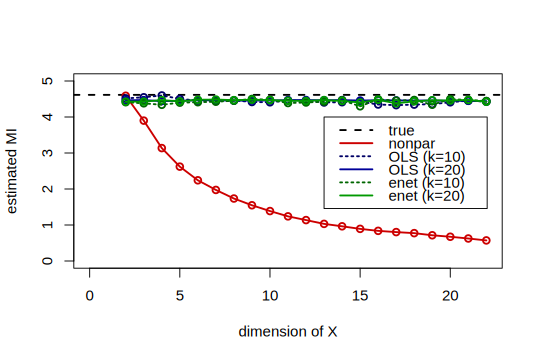
\includegraphics[scale = 0.8]{Figures/sim2a_fig1_edited.pdf}
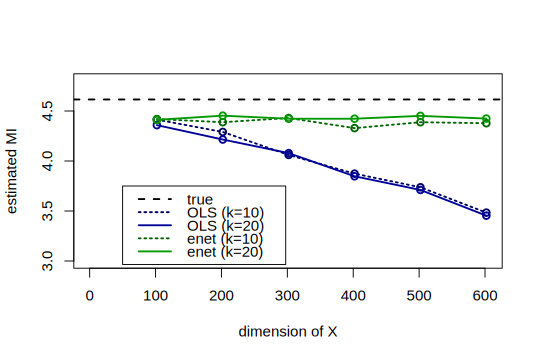
\includegraphics[scale = 0.8]{Figures/sim2a_fig3_edited.pdf}
\caption{Estimation of mutual information in simulated example.}
\label{fig:ch4_simulation}
\end{figure}

We will see additional examples in the next chapter, including a
simulation example involving a dense model.
 
% Chapter 5

\chapter{High-dimensional inference of mutual information} % Main chapter title

\label{Chapter5} % For referencing the chapter elsewhere, use \ref{Chapter1} 

\section{Motivation}

\subsection{Quantifying precision of decoding models}

\subsection{Kay et al. example}

\section{Setup}

\section{Theory}

\section{Estimator}

\section{Examples}


 
% Chapter 6

\chapter{Discussion} % Main chapter title

\label{Chapter6} % For referencing the chapter elsewhere, use \ref{Chapter1} 

In this thesis, we considered the problem of evaluating the quality of
a feature embedding, or representation $\vec{g}(\vec{x})$ using
side-information from a response $y$.  As we showed in the
introduction, the problem of supervised evaluation of representations
occurs in both machine learning and neuroscience; therefore, our work
is relevant for both areas, but also yields tools that may be useful
for other disciplines as well.

We investigated three closely related approaches for doing so: mutual
information $I(\vec{g}(\vec{X}); Y)$, average accuracy for randomized
classification, and identification accuracy.  The identification
accuracy is based on the same fundamental prediction task as
randomized classification, which is to assign a feature vector $X$ to
one of $k$ discrete classes.  Therefore, the average Bayes accuracy,
defined in Chapter 2, is an upper bound for both average accuracy for
randomized classification and identification accuracy.  The mutual
information can be linked, via Shannon's coding theorem, to the
decoding accuracy achievable using a random codebook, and therefore it
is not surprising that we can link mutual information to average Bayes
accuracy for randomized classification, as we showed in Chapter 4.

Thus, by combining all of these results, we can convert estimates of
average accuracy or estimates of identification accuracy into
estimates of mutual information.  This provides a useful tool for
several reasons.  One is that for the purpose of assessing
representations, both the average accuracy and the identification
accuracy have a dependence on an arbitrary tuning parameter $k$.  To
eliminate the dependence, we can convert either to an estimate of
mutual information, which can be interpreted without knowing $k$.  Of
course, the estimation procedure itself might still depend on the
choice of $k$, as we saw in the example of section
\ref{sec:real_data}--but it is possible that future work may provide a
remedy.

Secondly, for users interested in estimating the mutual information
$I(X; Y)$, the possibility of deriving new estimators of mutual
information from average accuracy or identification accuracy greatly
expands the arsenal of mutual information estimators.  This is because
one can exploit a variety of different types of problem-specific
assumptions, such as sparsity, in the training of the regression or
classification model used to compute average accuracy or
identification risk.

Thirdly, there is the interesting possibility of converting
$k_1$-class accuracy into an estimate of mutual information, and then
converting the estimated mutual information into an estimate of
$k_2$-class accuracy, for some $k_2 > k_1$.  We have not addressed
this possibility in the current work, but it provides an
information-based means of extrapolating classification accuracy,
which could be compared to the unbiased estimation method for the same
problem that we developed in Chapter 3.

On the other hand, one may choose to work with the average accuracy or
identification accuracy directly.  Rather than trying to eliminate the
parameter $k$, we can try to understand its effect.  For this purpose,
the theory of average accuracy (which also applies to identification
accuracy) developed in Chapter 3, is invaluable.  We see that the
$k$-class average accuracy is simply a $(k-1)$th moment of a
\emph{conditional accuracy} distribution; and this can be used to
estimate average accuracy at arbitrary $k$.  Understanding how the
average accuracy scales with $k$ also yields practical benefits: it
allows us to understand how recognition systems might scale under
larger problems, and it allows us to compare two different feature
representations on the basis of the entire average accuracy curve
rather than the average accuracy at a single $k$.

In the ideal case, however, the mutual information and average
accuracy curve give equivalent information--which is to say that the
mutual information is a perfect summary of the average accuracy curve.
We saw in Chapter 5 that such a situation occurs in a particular
high-dimensional limit where the true mutual information tends to a
constant.  This limit may be a good fit to many applied
high-dimensional problems.  However, in lower-dimensional problems,
there is a tradeoff between working with $k$-class average accuracy or
average identification directly, which are easy to estimate but which
depend on the choice of $k$, or getting rid of $k$ by converting to an
estimate of mutual information.

While we showed mathematically how mutual information is connected to
average accuracy and identification accuracy, from an intuitive
perspective, they can all be seen to correspond to some notion of
information-theoretic volume in the embedding space.  We already saw
how mutual information can be related to metric entropy in Chapter 1;
but the average accuracy (or equivalently, the identification
accuracy) can also be used to measure volume, if we define the
$\epsilon$-\emph{capacity} of an embedding to be the maximal number of classes $k$
where the average accuracy is above some threshold $\epsilon$.  This
concept of volume differs slightly from metric entropy or covering
numbers because it refers to the spacing properties of random sets of
points, rather than an optimized set of points.  Still, we expect that
the different ways of defining volume can all be connected in a more
formal sense, and we anticipate that lower or upper bounds of metric
entropy can be stated in terms of average Bayes accuracy or mutual
information.

Two obvious areas of development for our methods is to obtain (i)
formal checks of the assumptions (e.g. the high-dimensionality
assumption in Ch. 5) which our methods depend on, and (ii) to
characterize the quality of the estimators in a decision-theoretic
framework, and (iii) to develop interval estimates of mutual
information or $\epsilon$-capacity.  We have made initial progress
towards developing the understanding necessary to develop these
methods, e.g. the variance bounds on Bayes accuracy in Chapter 2.

Another important research direction would be to apply these
methods to more practical real-life examples.  Applications always
reveal surprising insights about what kind of models are needed, or
what kind of properties are most desirable for a statistical
procedure.  In this thesis, we discussed the use of our methods in
predicting the performance of face-recognition systems, understanding
the generalizability of neuroscience experiments, and estimating
mutual information in high-dimensional settings; further exploration
of any of these particular applications could motivate new refinements
and extensions of our methods, but there may also be many additional
applications where our ideas can be applied.

 

%----------------------------------------------------------------------------------------
%	THESIS CONTENT - APPENDICES
%----------------------------------------------------------------------------------------

\appendix % Cue to tell LaTeX that the following "chapters" are Appendices

% Include the appendices of the thesis as separate files from the Appendices folder
% Uncomment the lines as you write the Appendices

%% Appendix A

\chapter{Appendix for Chapter 1} % Main appendix title

\label{AppendixA} % For referencing this appendix elsewhere, use \ref{AppendixA}

\section{Proofs}


%% Appendix B

\chapter{Appendix for Chapter 2} % Main appendix title

\label{AppendixB} % For referencing this appendix elsewhere, use \ref{AppendixA}

\section{Proofs}


% Appendix C

\chapter{Appendix for Chapter 3} % Main appendix title

\label{AppendixC} % For referencing this appendix elsewhere, use \ref{AppendixA}

\section{Proofs}

\begin{lemma}\label{lemma:U_function}
Suppose $\pi$, $\{F_y\}_{y \in \mathcal{Y}}$ and marginal classifier
$\mathcal{F}$ satisfy the tie-breaking condition.  Take $x \in \mathcal{X}$.  Defining
$U_{y,\hat{F}_y}(x)$ as in \eqref{eq:U_function}, and defining the
random variable $U$ by
\[U = U_{Y, \hat{F}_Y}(x)\]
for $Y \sim \pi$, $\hat{F}_Y \sim \Pi_{Y, r}$,
the distribution of $U$ is uniform on $[0,1]$, i.e.
\[
\Pr[U \leq u] = \text{max}\{u, 1\}.
\]
\end{lemma}

\textbf{Proof of Lemma A.1.}

Define the variable $Z = \mathcal{M}(\hat{F}_Y)(x)$ for $Y \sim \pi$.
By the tie-breaking condition, $Z$ has a continuous density on $[0,1]$.
Consider the survivor function of $Z$, $g(z) = \Pr[Z \geq z]$.  From
the definition \eqref{eq:U_function}, we see that 
\[
U = g(\mathcal{M}(\hat{F}_Y)(x)) = g(Z).
\]
Now note that the survivor function of any continuous random variable,
when applied to itself, is uniformly distributed.
$\Box$

% Appendix D

\chapter{Appendix for Chapter 4} % Main appendix title

\label{AppendixD} % For referencing this appendix elsewhere, use \ref{AppendixA}

\section{Proofs}


\begin{lemma}\label{lemma:technical1}
Let $f(t)$ be an increasing function from $[a, b] \to \mathbb{R}$, where $a < b$,
and let $g(t)$ be a bounded continuous function from $[a, b] \to \mathbb{R}$.
Define the set
\[
A = \{t: f(t) \neq g(t)\}.
\]
Then, we can write $A$ as a countable union of intervals
\[
A = \bigcup_{i=1}^\infty A_i
\]
where $A_i$ are mutually disjoint intervals, with $\inf A_i < \sup
A_i$, and for each $i$, either $f(t) > g(t)$ for all $t \in A_i$ or
$f(t) < g(t)$ for all $t \in A_i$.
\end{lemma}

\textbf{Proof of Lemma \ref{lemma:technical1}.} 

The function $h(t) = f(t) - g(t)$ is measurable, since all increasing
functions are measurable.  Define $A^+ = \{t: f(t) > g(t)\}$ and $A^-
= \{t: f(t) < g(t)\}$.  Since $A^+$ and $A^-$ are measurable subsets
of $\mathbb{R}$, they both admit countable partitions consisting of open, closed, or half-open
intervals.  Let $\mathcal{H}^+$ be the collection of all partitions of $A^+$ consisting of such intervals.
There exists a least refined partition $\mathcal{A}^+$ within $\mathcal{H}^+$.
Define $\mathcal{A}^-$ analogously, and let
\[
\mathcal{A} = \mathcal{A}^+ \cup \mathcal{A}^-
\]
and enumerate the elements
\[
\mathcal{A} = \{A_i\}_{i=1}^\infty.
\]

We claim that the partitions $\mathcal{A}^+$ and $\mathcal{A}^-$ have
the the property that for all $t \in A^\pm$, ther interval
$I \in \mathcal{A}^\pm$ containing $t$ has endpoints $l \leq u$
defined by
\[
l = \inf_{x \in [a,b]} \{x: \text{Sign}(h([x, t])) = \{\text{Sign}(h(t))\} \}
\]
and
\[
u = \sup_{x \in a[,b]} \{x: \text{Sign}(h([t, x])) = \{\text{Sign}(h(t))\}\}.
\]
We prove the claim for the partition $\mathcal{A}^+$.  Take $t \in
A^+$ and define $l$ and $u$ as above.  It is clear that $(l, u) \in
A^+$, and furthermore, there is no $l' < l$ and $u' > u$ such that
$(l', x) \in A^+$ or $(x, u') \in A^+$ for any $x \in I$.  Let
$\mathcal{H}$ be any other partition of $A^+$.  Some disjoint union of
intervals $H_i \in \mathcal{H}$ necessarily covers $I$ for $i =
1,...$, and we can further require that none of the $H_i$ are disjoint
with $I$.  Since each $H_i$ has nonempty intersection with $I$, and
$I$ is an interval, this implies that $\cup_i H_i$ is also an
interval.  Let $l'' \leq u''$ be the endpoints of $\cup_i H_i$ Since
$I \subseteq \cup_i H_i$, we have $l'' \leq l \leq u \leq u''$.
However, since also $I \in A^+$, we must have $l \leq l'' \leq
u'' \leq u$.  This implies that $l''=l$ and $u''=u$.  Since $\cup_i
H_i = I$, and this holds for any $I \in \mathcal{A}^+$, we conclude
that $\mathcal{H}$ is a refinement of $\mathcal{A}^+$. The proof of
the claim for $\mathcal{A}^-$ is similar.

It remains to show that there are not isolated points in
$\mathcal{A}$, i.e. that for all $I \in \mathcal{A}$ with endpoints
$l \leq u$, we have $l < u$.  Take $I \in \mathcal{A}$ with endpoints
$l \leq u$ and let $t = \frac{l+u}{2}$.  By definition, we have
$h(t) \neq 0$.  Consider the two cases $h(t) > 0$ and $h(t) < 0$.

If $h(t) > 0$, then $t' = g^{-1}(h(t)) > t$, and for all $x \in [t,
t']$ we have $h(x) > 0$.  Therefore, it follows from definition that
$[t, t'] \in I$, and since $l \leq t < t' \leq u$, this implies that
$l < u$.  The case $h(t) < 0$ is handled similarly. $\Box$

\begin{lemma}\label{lemma:technical2}
Let $f(t)$ be a measurable function from $[a,b] \to \mathbb{R}$, where $a < b.$
Then there exists sets $\mathcal{B}_0$ and $\mathcal{B}_1$, satisfying the following properties:
\begin{itemize}
\item  $\mathcal{B} = \mathcal{B}_0 \cup \mathcal{B}_1$ is countable partition of $[a,b]$,
\item  $f(t)$ is constant on all $B \in \mathcal{B}_0$, but not constant on any proper superinterval $B' \supset B$, and
\item $B \in \mathcal{B}_1$ contains no positive-length subinterval where $f(t)$ is constant.
\end{itemize}
\end{lemma}

\textbf{Proof of Lemma \ref{lemma:technical2}.} 
To construct the interval, define
\[
l(t) = \inf \{x \in [0,1]: f([x,t]) = \{f(t)\}\}
\]
\[
u(t) = \sup \{x \in [0,1]: f([t,x]) = \{f(t)\}\},
\]
Let $B_0$ be the set of all $t$ such that $l(t) < u(t)$,
and let $B_1$ be the set of all $t$ such that $l(t) = t = u(t)$.
For all $t \in B_0$, define
\[
I(t) = (l(t), u(t)) \cup \{x \in \{l(t), u(t)\}: f(x) = f(t)\}.
\]
Then we claim
\[
\mathcal{B}_0 = \{I(t): t \in B_0\}
\]
is a countable partition of $B_0$.  The claim follows since the
members of $\mathcal{B}_0$ are disjoint intervals of nonzero length,
and $B_0$ has finite length.    It follows from definition that for any $B \in B_0$, that $f$ is not
constant on any proper superinterval $B' \supset B$.

Meanwhile, let $\mathcal{B}_1$ be a countable partition of $B_1$ into
intervals.

Next, we show that for all $I \in \mathcal{B}_1$, $I$ does not contain
a subinterval $I'$ of nonzero length such that $f$ is constant on
$I'$.  Suppose to the contrary, we could find such an interval $I$ and
subinterval $I'$.  Then for any $t \in I'$, we have $t \in B_0$.
However, this implies that $t \notin B_1$, a contradiction.

Since $t \in [a,b]$ belongs to either $B_0$ or $B_1$,
letting $\mathcal{B} = \mathcal{B}_0 \cup \mathcal{B}_1$
yields the desired partition of $[a,b]$. $\Box$.

\begin{lemma}\label{lemma:mono_entropy}
Define an exponential family on $[0,1]$ by the density function
\[
q_\beta(t) = \exp[\beta t^{k-1} - \log Z(\beta)]
\]
where
\[
Z(\beta) = \int_0^1 \exp[\beta t^{k-1}] dt.
\]
Then, the negative entropy
\[
I(\beta) = \int_0^1 q_\beta(t) \log q_\beta(t) dt
\]
is decreasing in $\beta$ on the interval $(-\infty, 0]$.
and increasing on the interval $[0, \infty)$.

Furthermore, for any $\iota \in (0,\infty)$, there exist two solutions
to $I(\beta) = \iota$: one positive and one negative.
\end{lemma}

\textbf{Proof of Lemma \ref{lemma:mono_entropy}.}

Define $\beta(\mu)$ as the solution to
\[
\mu = \int_0^1 t q_\beta(t) dt.
\]
By [Wainwright and Jordan 2008], the function $\beta(\mu)$ is
well-defined.  Furthermore, since the sufficient statistic $t^{k-1}$
is increasing in $t$, it follows that $\beta(\mu)$ is increasing.

Define the negative entropy as a function of $\mu$,
\[
N(\mu) = \int_0^1 q_{\beta(\mu)}(t) \log q_{\beta(\mu)}(t) dt.
\]

By Theorem 3.4 of [Wainwright and Jordan 2008], $N(\mu)$ is convex in
$\mu$.  We claim that the derivative of $N(\mu) = 0$ at $\mu
= \frac{1}{2}$.  This implies that $N(\mu)$ is decreasing in $\mu$ for
$\mu \leq \frac{1}{2}$ and increasing for $\mu \geq \frac{1}{2}$.
Since $I(\beta(\mu)) = N(\mu)$, $\beta$ is increasing in $\mu$, and
$\beta(\frac{1}{2}) = 0$, this implies that $I(\beta)$ is decreasing
in $\beta$ for $\beta \leq 0$ and increasing for $\beta \geq 0$.

We will now prove the claim.  Write
\[
\frac{d}{d\mu} N(\mu)\bigg|_{\mu = 1/2} = \frac{d}{d\beta} I(\beta(\mu)) \bigg|_{\beta = 0} \frac{d\beta}{d\mu} \bigg|_{\mu = 1/2}.
\]
We have
\[
\frac{d}{d\beta} I(\beta) = \beta \int q_\beta t^{k-1} dt - \log Z(\beta).
\]
Meanwhile, $Z(0) = 1$ so $\log Z(0) = 0$.  Therefore,
\[
\frac{d}{d\beta} I(\beta) \bigg|_{\beta = 0} = 0.
\]
This implies that $\frac{d}{d\mu} N(\mu) |_{\mu = 1/2} = 0$, as needed.  

For the final statement of the lemma, note that $I(0) = 0$ since $q_0$ is the uniform distribution.
Meanwhile, since $q_\beta$ tends to a point mass as either $\beta \to \infty$ or $\beta \to -\infty$,
we have 
\[
\lim_{\beta \to \infty} I(\beta) = \lim_{\beta \to -\infty} I(\beta) = \infty.
\]
And, as we can check that $I(\beta)$ is continuous in $\beta$, this means that
\[
I((-\infty, 0]) = I([0,\infty)) = [0, \infty)
\]
by the mean-value theorem.  Combining this fact with the monotonicity
of $I(\beta)$ restricted to either the positive and negative half-line
yields the fact that for any $\iota > 0$, there exists $\beta_1 < 0
< \beta_2$ such that $I(\beta_1) = I(\beta_2) = \iota$.  $\Box$.

\begin{lemma}\label{lemma:variational}
For any measure $G$ on $[0, \infty]$,
let $G^k$ denote the measure defined by
\[
G^k(A) = G(A)^k,
\]
and define
\[
E[G] = \int x dG(x).
\]
\[
I[G] = \int x \log x dG(x)
\]
and
\[
\psi_k[G] = \int x d(G^k)(x).
\]
Then, defining $Q_c$ and $c_\iota$ as in Theorem 1, we have
\[
\sup_{G: E[G] = 1, I[G] \leq \iota} \psi_k[G] = \int_0^1 Q_{c_\iota}(t) t^{k-1} dt.
\]
Furthermore, the supremum is attained by a measure $G$ that has cdf
equal to $Q_c^{-1}$, and thus has a density $g$ with respect to
Lesbegue measure.
\end{lemma}

\textbf{Proof of Lemma \ref{lemma:variational}.} 

Consider the quantile function $Q(t) = \inf_{x \in [0,1]}: G((-\infty,
x]) \geq t.$ $Q(t)$ must be a monotonically increasing function from
$[0,1]$ to $[0,\infty).$ Let $\mathcal{Q}$ denote the collection of
all such quantile functions.

We have
\[
E[G] = \int_0^1 Q(t) dt
\]
\[
\psi_k[G] = \int_0^1 Q(t) x^{k-1} dt.
\]
and
\[
I[G] = \int_0^1 Q(t) \log Q(t) dt.
\]

For any given $\iota$, let $P_\iota$ denote the class of probability
distributions $G$ on $[0, \infty]$ such that $E[G]=1$ and
$I[G] \leq \iota.$  From Markov's inequality, for any $G \in P_\iota$
we have
\[
G([x, \infty]) \leq x^{-1}
\]
for any $x \geq 0$, hence $P_\iota$ is tight.  From tightness, we
conclude that $P_\iota$ is closed under limits with respect to weak
convergence.  Hence, since $\psi_k$ is a continuous function, there
exists a distribution $G^* \in P_\iota$ which attains the supremum
\[\sup_{G \in P_\iota} \psi_k[G].\]
Let $\mathcal{Q}_\iota$ denote the collection of quantile functions of
distributions in $P_\iota.$ Then, $\mathcal{Q}_\iota$ consists of monotonic functions
$Q: [0,1] \to [0, \infty]$ which
satisfy
\[
E[Q] = \int_0^1 Q(t) dt = 1,
\]
and
\[
I[Q] = \int_0^1 Q(t) \log Q(t) dt \leq \iota.
\]
Let $\mathcal{Q}$ denote the collection of \emph{all} quantile functions from measures on $[0,\infty]$.
And letting $Q^*$ be the quantile function for $G^*$, we have that
$Q^*$ attains the supremum
\begin{equation}\label{eq:constrained_optim}
\sup_{Q \in \mathcal{Q}_\iota} \phi_k[Q] = \sup_{Q \in \mathcal{Q}_\iota} \int_0^1 Q(t) t^{k-1} dt.
\end{equation}
Therefore, there exist Lagrange multipliers
$\lambda \geq 0$ and $\nu \geq 0$ such that defining
\[
\mathcal{L}[Q] = -\phi_k[Q] + \lambda E[Q] + \nu I[Q]= \int_0^1 Q(t) (-t^{k-1} + \lambda + \nu \log Q(t)) dt,
\]
$Q^*$ attains the infimum of $\mathcal{L}[Q]$ over \emph{all} quantile functions,
\[
\mathcal{L}[Q^*] = \inf_{Q \in \mathcal{Q}}\mathcal{L}[Q].
\]
The global minimizer $Q^*$ is also necessarily a stationary point:
that is, for any perturbation function $\xi: [0,1] \to \mathbb{R}$
such that $Q^* + \xi \in \mathcal{Q}$, we have $\mathcal{L}[Q^*]\leq \mathcal{L}[Q^* + \xi]$.
For sufficiently small $\xi$, we have
\begin{equation}\label{eq:Lperturb}
\mathcal{L}[Q + \xi] \approx \mathcal{L}[Q] + \int_0^1 \xi(t) (-t^{k-1} + \lambda + \nu + \nu \log Q(t)) dt.
\end{equation}
Define
\begin{equation}\label{eq:nablaQ}
\nabla \mathcal{L}_{Q^*}(t) = -t^{k-1} + \lambda + \nu + \nu \log Q(t).
\end{equation}
The function $\nabla \mathcal{L}_{Q^*}(t)$ is a \emph{functional derivative} of the Lagrangian.
Note that if we were able to show that $\nabla \mathcal{L}_{Q^*}(t) = 0$,
this immediately yields
\begin{equation}\label{eq:Qstareq}
Q^*(t) = \exp[-1 -\lambda\nu^{-1} + \nu^{-1}  t^{k-1}].
\end{equation}
At this point, we know that the right-hand side of \eqref{eq:Qstareq}
gives a stationary point of $\mathcal{L}$, but we cannot be sure that
it gives the global minimzer.  The reason is because the optimization
occurs on a constrained space.  We will show that \eqref{eq:Qstareq}
indeed gives the global minimizer $Q^*$, but we do so by showing that
the set of points $t$ where $\nabla \mathcal{L}_{Q^*}(t) \neq 0$ is of
zero measure.  Since sets of zero measure don't affect the integrals
defining the optimization problem \eqref{eq:constrained_optim}, we
conclude there exists a global optimal solution with
$\nabla \mathcal{L}_{Q^*}(t) = 0$ everywhere, which is therefore given
explicitly by \eqref{eq:Qstareq} for some $\lambda \in \mathbb{R}$, $\nu \geq 0.$

We will need the following result: that for $\iota
> 0$, any solution to \eqref{eq:constrained_optim} satisfies
$\phi_k[Q] < 1$.  This follows from the fact that
\[
E[Q] - \phi_k[Q] = \int_0^1 (1-t^{k-1}) Q(t) dt,
\]
where the term $(1-t^{k-1})$ is negative, except for the one point $t
= 1$.  Therefore, in order for $\phi_k[Q] = 1 = E[Q]$, we must have
$Q(t) = 0$ for $t < 1$.  However, this yields a contradiction since
$Q(t) = 0$ for $t < 1$ implies that $E[Q] = 0$, a violation of the
hard constraint $E[Q] = 1$.

Let us establish that $\nu > 0$: in other words, the constraint $I[Q]
= \iota$ is tight.  Suppose to the contrary, that for
some $\iota > 0$, the global optimum $Q^*$ minimizes a Lagrangian with
$\nu = 0$.  Let $\phi^* = \phi_k[Q^*] < 1.$ However, if we define
$Q_\kappa(t) = I\{t \geq 1 - \frac{1}{\kappa}\} \kappa$, we have
$E[Q_\kappa] = 1$, and also for some sufficiently large $\kappa > 0$,
$\phi_k[Q_\kappa] > \phi^*$.  But since the Lagrangian lacks a term
corresponding to $I[Q]$, we conclude that $\mathcal{L}[Q_\kappa]
< \mathcal{L}[Q^*]$, a contradiction.

The rest of the proof proceeds as follows.  We will use
Lemmas \ref{lemma:technical1} and \ref{lemma:technical2} to define a
decomposition $A = D_0 \cup D_1 \cup D_2$, where $D_2$ is of measure
zero.  First, we show that assuming the existence of $t \in D_0$
yields a contradiction, and hence $D_0 = \emptyset$.  Then, again
using argument from contradiction we establish that $D_1 = \emptyset$.
Finally, since $D_2$ is a set of zero measure, this allows us to
conclude that the $Q^*(t) = 0$ on all but a set of zero measure.

We will now apply the Lemmas to obtain the necessary ingredients for
constructing the sets $D_i$.  Since $\nabla \mathcal{L}_{Q^*}(t)$ is a difference
between an increasing function and a continuous stricly increasing
function, we can apply Lemma \ref{lemma:technical1} to conclude that
there exists a countable partition $\mathcal{A}$ of the set
$A: \{t \in [0,1]: \nabla \mathcal{L}_{Q^*}(t) \neq 0\}$ into intervals such that
for all $J \in \mathcal{A}$, $|\text{Sign}(\nabla Q^*(J))| = 1$ and
$\inf J < \sup I$ .  Applying Lemma \ref{lemma:technical2} we get a
countable partition $\mathcal{B} = \mathcal{B}_0 \cup \mathcal{B}_1$
of $[0,1]$ so that each element $J \in \mathcal{B}_0$ is an interval
such that $\nabla \mathcal{L}_{Q^*}(t)$ is constant on $J$, and furthermore is not
properly contained in any interval with the same property, and each
element $J \in \mathcal{B}_1$ is an interval, such that $J$ contains
no positive-length subinterval where $\nabla \mathcal{L}_{Q^*}(t)$ is constant.
Also define $B_i$ as the union of the sets in $\mathcal{B}_i$ for $i =
0,1$.

Note that $B_0$ is necessarily a subset of $A$.  That is because if
$\nabla \mathcal{L}_{Q^*}(t) = 0$ on any interval $J$, then that $Q^*(t)$ is
necessarily not constant on the interval.  

We will construct a new countable partition of $A$, called $\mathcal{D}$.
The partition $\mathcal{D}$ is constructed by taking the union of three families of intervals,
\[
\mathcal{D} = \mathcal{D}_0 \cup \mathcal{D}_1 \cup \mathcal{D}_2.
\]
Define $D_i$ to be the union of intervals in $\mathcal{D}_i$ for $i = 0,1,2$.

Define $\mathcal{D}_0 = \mathcal{B}_0$,
Define a countable partition $\mathcal{D}_1$ by
\[
\mathcal{D}_1 = \{J \cap L: J \in \mathcal{A}, L \in \mathcal{B}_1, \text{ and } |L| > 1\},
\]
in order words, $\mathcal{D}_1$ consists of positive-length intervals where $\nabla
Q^*(t)$ is entirely positive or negative and is not constant.
Define
\[
\mathcal{D}_2 = \{J \in \mathcal{B}_1: J \subset A \text{ and } |J| = 1 \},
\]
i.e. $\mathcal{D}_2$ consists of isolated points in $A$.

One verifies that $\mathcal{D}$ is indeed a partition of $A$ by
checking that $D_0 = B_0$, $D_1 \cup D_2 = B_1 \cap A$, so that
$D_0 \cup D_2 \cup D_2 = A$: it is also easy to check that elements of
$\mathcal{D}$ are disjoint.  Furthermore, as we mentioned earlier, the
set $D_2$ is indeed of zero measure, since it consists of countably
many isolated points.

Now we will show that the existence of $t \in D_0$ implies a contradiction.
Take $t \in D$ for $D \in \mathcal{D}_0$, and let $a = \inf D$ and $b
= \sup D$.  Define
\[
\xi^+ = I\{t \in D\} (Q^*(b) - Q^*(t))
\]
and
\[
\xi^- = I\{t \in D\} (Q^*(a) - Q^*(t)).
\]
Observe that $Q + \epsilon \xi^+ \in \mathcal{Q}$ and $Q
+ \epsilon \xi^- \in \mathcal{Q}$ for any $\epsilon \in [0,1]$.  Now,
if $\nabla \mathcal{L}_{Q^*}(t)$ is strictly positive on $D$, then for some
$\epsilon > 0$ we would have $\mathcal{L}[Q^* + \epsilon \xi^-]
< \mathcal{L}[Q^*]$, a contradiction.  A similar argument with $\xi^+$
shows that $\nabla \mathcal{L}_{Q^*}(t)$ cannot be strictly negative on $D$ either.
From this pertubation argument, we conclude that $\nabla \mathcal{L}_{Q^*}(t) = 0$.
Since this argument applies for all $t \in D_0$, we conclude that $D_0
= \emptyset$: therefore, on the set $[0,1] \setminus (D_1 \cup D_2)$,
we have $\nabla \mathcal{L}_{Q^*}(t) = 0.$

The following observation is needed for the next stage of the proof.
If we look at the function $Q^*(t)$, then up so sets of neglible
measure, it is given by the expression \eqref{eq:Qstareq} on the set
$[0,1]\setminus D_1$, and it is piecewise constant in-between.  But
since \eqref{eq:Qstareq} gives a strictly increasing function, and
since $Q^*$ is increasing, this implies that $Q^*$ is discontinuous at
the boundary of $D_1$.

Now we are prepared to show that $\nabla \mathcal{L}_{Q^*}(t) = 0$ for $t \in D_1$.
Take $t \in D$ for $D \in \mathcal{D}_1$, and let $a = \inf D$ and $b
= \sup D$.  From the previous argument, there is a discontinuity at
both $a$ and $b$, so that $\lim_{u \to a^-} Q(u) < Q(t) < \lim_{u \to
b^+} Q(u)$.  Therefore, for any $\xi(t)$ which is increasing on $D$
and zero elsewhere, there exists $\epsilon > 0$ such that $\nabla Q^*
+ \epsilon \xi \in \mathcal{Q}.$ It remains to find such a
perturbation $\xi$ such that $\mathcal{L}[Q + \epsilon \xi]
< \mathcal{L}[Q]$.

Also, since by definition $\nabla \mathcal{L}_{Q^*}(t)$ is constant on $D$, follows from\eqref{eq:nablaQ} that
$\nabla Q^*$ is strictly decreasing, and thus either
\begin{itemize}
\item Case 1: $\nabla \mathcal{L}_{Q^*}(t) \geq 0$ on $D$,
\item Case 2: $\nabla \mathcal{L}_{Q^*}(t) \leq 0$ on $D$, or
\item Case 3: $\nabla \mathcal{L}_{Q^*}(t) \geq 0$ for all $t \in D \cap [a, t_0]$ and $\nabla \mathcal{L}_{Q^*}(t) \leq 0$ for all $t \in D \cap [t_0, b]$.
\end{itemize}

Depending on the case, we construct a suitable perturbation $\xi$:
\begin{itemize}
\item Case 1: Construct $\xi(t) = -I\{t \in D\}$.
\item Case 2: Construct $\xi(t) = I\{t \in D\}$
\item Case 2: Construct
\[
\xi(t) = \begin{cases}
-1 & \text{ for }t \in D \cap [a, t_0],\\
0 & \text{ otherwise. }
\end{cases}
\]
\end{itemize}
In all three cases, given the corresponding construction for $\xi(t)$ we get
\[
\int_0^1 \xi(t) \nabla \mathcal{L}_{Q^*}(t) dt < 0.
\]
Therefore, from \eqref{eq:Lperturb}, there exists some $\epsilon > 0$
such that $\mathcal{L}[Q + \epsilon \xi] < \mathcal{L}[Q]$, a
contradiction.  Again, since the contradiction applies for all $t \in
D_1$, we conclude that $D_1 = \emptyset$.

By now we have established that a global optimum
for \eqref{eq:constrained_optim} exists, and is given
by \eqref{eq:Qstareq} for some $\lambda \in \mathbb{R}$, $\nu > 0$.  It remains
to determine the values of $\lambda$ and $\nu$.

Reparameterize $\alpha = \exp[-1-\lambda\nu^{-1}]$ and $\beta = \nu^{-1}$.
Therefore,
\[
Q^*(t) = \alpha \exp[\beta t^{k-1}]
\]
for $\alpha > 0$, $\beta > 0$.  There is a one-to-one mapping from
$(\alpha, \beta) \in (0, \infty)^2$ to $(\lambda, \nu) \in
\mathbb{R} \times (0,\infty)$.

Now, from the constraint
\[
1 = E[Q^*] = \int_0^1 \alpha \exp[\beta t^{k-1}] dt.
\]
we conclude that
\[
\alpha = \frac{1}{\int_0^1 \exp[\beta t^{k-1}] dt.}
\]
Therefore, we have reduced the set of possible solutions $Q^*$ to a one-parameter family,
\[
Q^*(t) = \frac{\exp[\beta t^{k-1}]}{Z(\beta)}.
\]
where
\[
Z(\beta) = \int_0^1 \exp[\beta t^{k-1}] dt.
\]

Next, note that
\[
I[Q^*] = \int_0^1 Q^*(t) \log Q^*(t) = \beta \mu_\beta - \log Z(\beta),
\]
as a function of $\beta$, is completely characterized by Lemma \ref{lemma:mono_entropy}.
Let us define $c_\iota$ as the unique positive solution to the equation
\[
c_\iota \mu_{c_\iota} - \log Z(c_\iota) = \iota
\]
given by Lemma \ref{lemma:mono_entropy}.
We therefore have
\[
Q^*(t) = \frac{\exp[c_\iota t^{k-1}]}{\int_0^1 \exp[c_\iota t^{k-1}]},
\]
as needed. $\Box$


\begin{lemma}\label{lemma:concave}
The map
\[
\iota \to \int_0^1 Q_{c_\iota}(t) t^{k-1} dt
\]
is concave in $\iota > 0$.
\end{lemma}

\textbf{Proof of Lemma \ref{lemma:concave}.}
It is equivalent to show that the inverse function
\[
C^{-1}_k(p) = \inf_{G: E[G] = 1, \phi_k[G] = p} I[G]
\]
is convex.  Let $p_1, p_2 \in [0,1]$.  From
lemma \ref{lemma:variational}, we can find measures $G_1$, $G_2$ on
$[0,\infty)$ which minimize $I[G_i]$ subject to $E[G_i] = 1$ and
$\phi_k[G_i] = p_i$.  Define the measure
\[
H = \frac{G_1 + G_2}{2}.
\]
Since $\phi_k$ is a linear functional,
\[
\phi_k[H] = \frac{\phi_k[G_1] + \phi_k[G_2]}{2} = \frac{p_1 + p_2}{2}.
\]
But since $I$ is a convex functional,
\[
I[H] \leq \frac{I[G_1] + I[G_2]}{2}.
\]

Therefore,
\[
C^{-1}_k\left(\frac{p_1 + p_2}{2}\right) \leq I[H] = \frac{I[G_1] + I[G_2]}{2} = \frac{C^{-1}_k(p_1) + C^{-1}_k(p_2)}{2}.
\]
$\Box$.

%% Appendix E

\chapter{Appendix for Chapter 5} % Main appendix title

\label{AppendixE} % For referencing this appendix elsewhere, use \ref{AppendixA}

\section{Proofs}




 

\printbibliography[heading=bibintoc]

\end{document}

%% Normally the \chapter and any text would be in a separate file and included.

%% for Bibliography I would recommend a separate .bib file (bibtex) instead of inline as here.
%\nocite{astl2,perry1,pollardsag1}
%\nocite{*}
    \bibliographystyle{plain}
%    \bibliography{suthesis}

\begin{thebibliography}{1}

\bibitem{revelation}
{John of Patnos}.
\newblock Revelation of {St.} {John}.
\newblock In {\em Bible}. King James, 1611.

\bibitem{genesis}
Moses.
\newblock Genesis.
\newblock In {\em Bible}. King James, 1611.

\bibitem{preacher}
Preacher.
\newblock Ecclesiastes.
\newblock In {\em Bible}. King James, 1611.

\end{thebibliography}


\end{document}
